% !TEX root = ThesisGchatzi.tex

\subsection{Experimental Evaluation}
\label{subsec:local_sim_join_exp}

\graphicspath{{Papers/SSTD2019/}{Papers/SIGSpatial2019/}}

\subsubsection{Experimental Setup}
\label{subsec:evaluation_setup_join}
We evaluate the performance of our methods on pair and bundle discovery both qualitatively and quantitatively. We compare our checkpoint (CP) scan approaches for each problem with the respective sweep line (SL) methods. We use the water real-world dataset also used for experimental evaluation in Section~\ref{sec:exp_btsr} and a synthetic dataset, as listed in Table~\ref{tab:datasets_join}. The latter is consisted of 50,000 time series, each with a length of 1,000 timestamps. So, this dataset contains 50 million data points in total. The dataset was generated in a similar manner to the synthetic dataset used in \cite{keogh1999indexing}.

\begin{table}[ht]
\centering
\caption{Datasets used in the experiments.}
\begin{small}
\begin{tabular}{lcc} 
\hline
{\em Dataset} & {\em Size} & {\em Time series length} \\
\hline
Water & 822 & 168  \\
Synthetic & 50,000 & 1,000 \\
\hline
\end{tabular}
\end{small}
\label{tab:datasets_join}
\end{table}

All experiments were conducted on a Dell PowerEdge M910 with 4 Intel Xeon E7-4830 CPUs, each containing 8 cores clocked at 2.13GHz, 256 GB RAM and a total storage space of 900 GB.

\subsubsection{Evaluation Results}
\label{subsec:exp_results}
We conducted two sets of experiments, using the water and synthetic datasets. The water dataset was used for qualitative and quantitative assessment of our methods on pair and bundle discovery, while the synthetic dataset was used for efficiency evaluation.

\subsubsubsection{Pair and Bundle Discovery over Real Data}
\label{subsubsec:pair_bundle}
We performed several experiments using the water dataset for various parameter values to detect pairs and bundles using both the SL and CP approaches. The dataset was \textit{$z$-normalized} to eliminate amplitude discrepancies among time series and focus on structural similarity.

To evaluate our methods against different parameters, we performed preliminary tests to extract ranges of values where the algorithms would return a reasonable number of results. Table \ref{tab:parameters1_join} lists the range of values for the parameters used for bundle and pair discovery tests (recall that parameter $\mu$ is not applicable in pair discovery); default values are in bold. Parameter $\delta$ is expressed as a percentage of the duration of the time series, $\epsilon$ is expressed as a percentage of the value range (i.e., difference $max-min$ in values encountered across the dataset) and $\mu$ is expressed as a percentage of the number of time series in the dataset.

\begin{table}[!ht]
\centering
\caption{Parameters for tests over the water dataset}
\begin{small}
\begin{tabular}{lc} 
\hline
{\em Parameter} &{\em Values} \\
\hline
$\delta$ (\% of time series length, i.e., 168) & 6\%, 5\%, \textbf{6\%}, 7\%, 8\% \\
$\epsilon$ (\% of value range, i.e., approx 11.4) & 4\%, 5\%, \textbf{6\%}, 7\%, 8\% \\
$\mu$ (\% of dataset size, i.e., 822) & 0.5\%, 0.75\%, \textbf{1\%}, 1.25\%, 1.5\% \\
\hline
\end{tabular}
\end{small}
\label{tab:parameters1_join}
\end{table}

\paragraph{Varying $\delta$}
\begin{figure}[!ht]
 \centering
 \subfloat[Bundle discovery execution time]{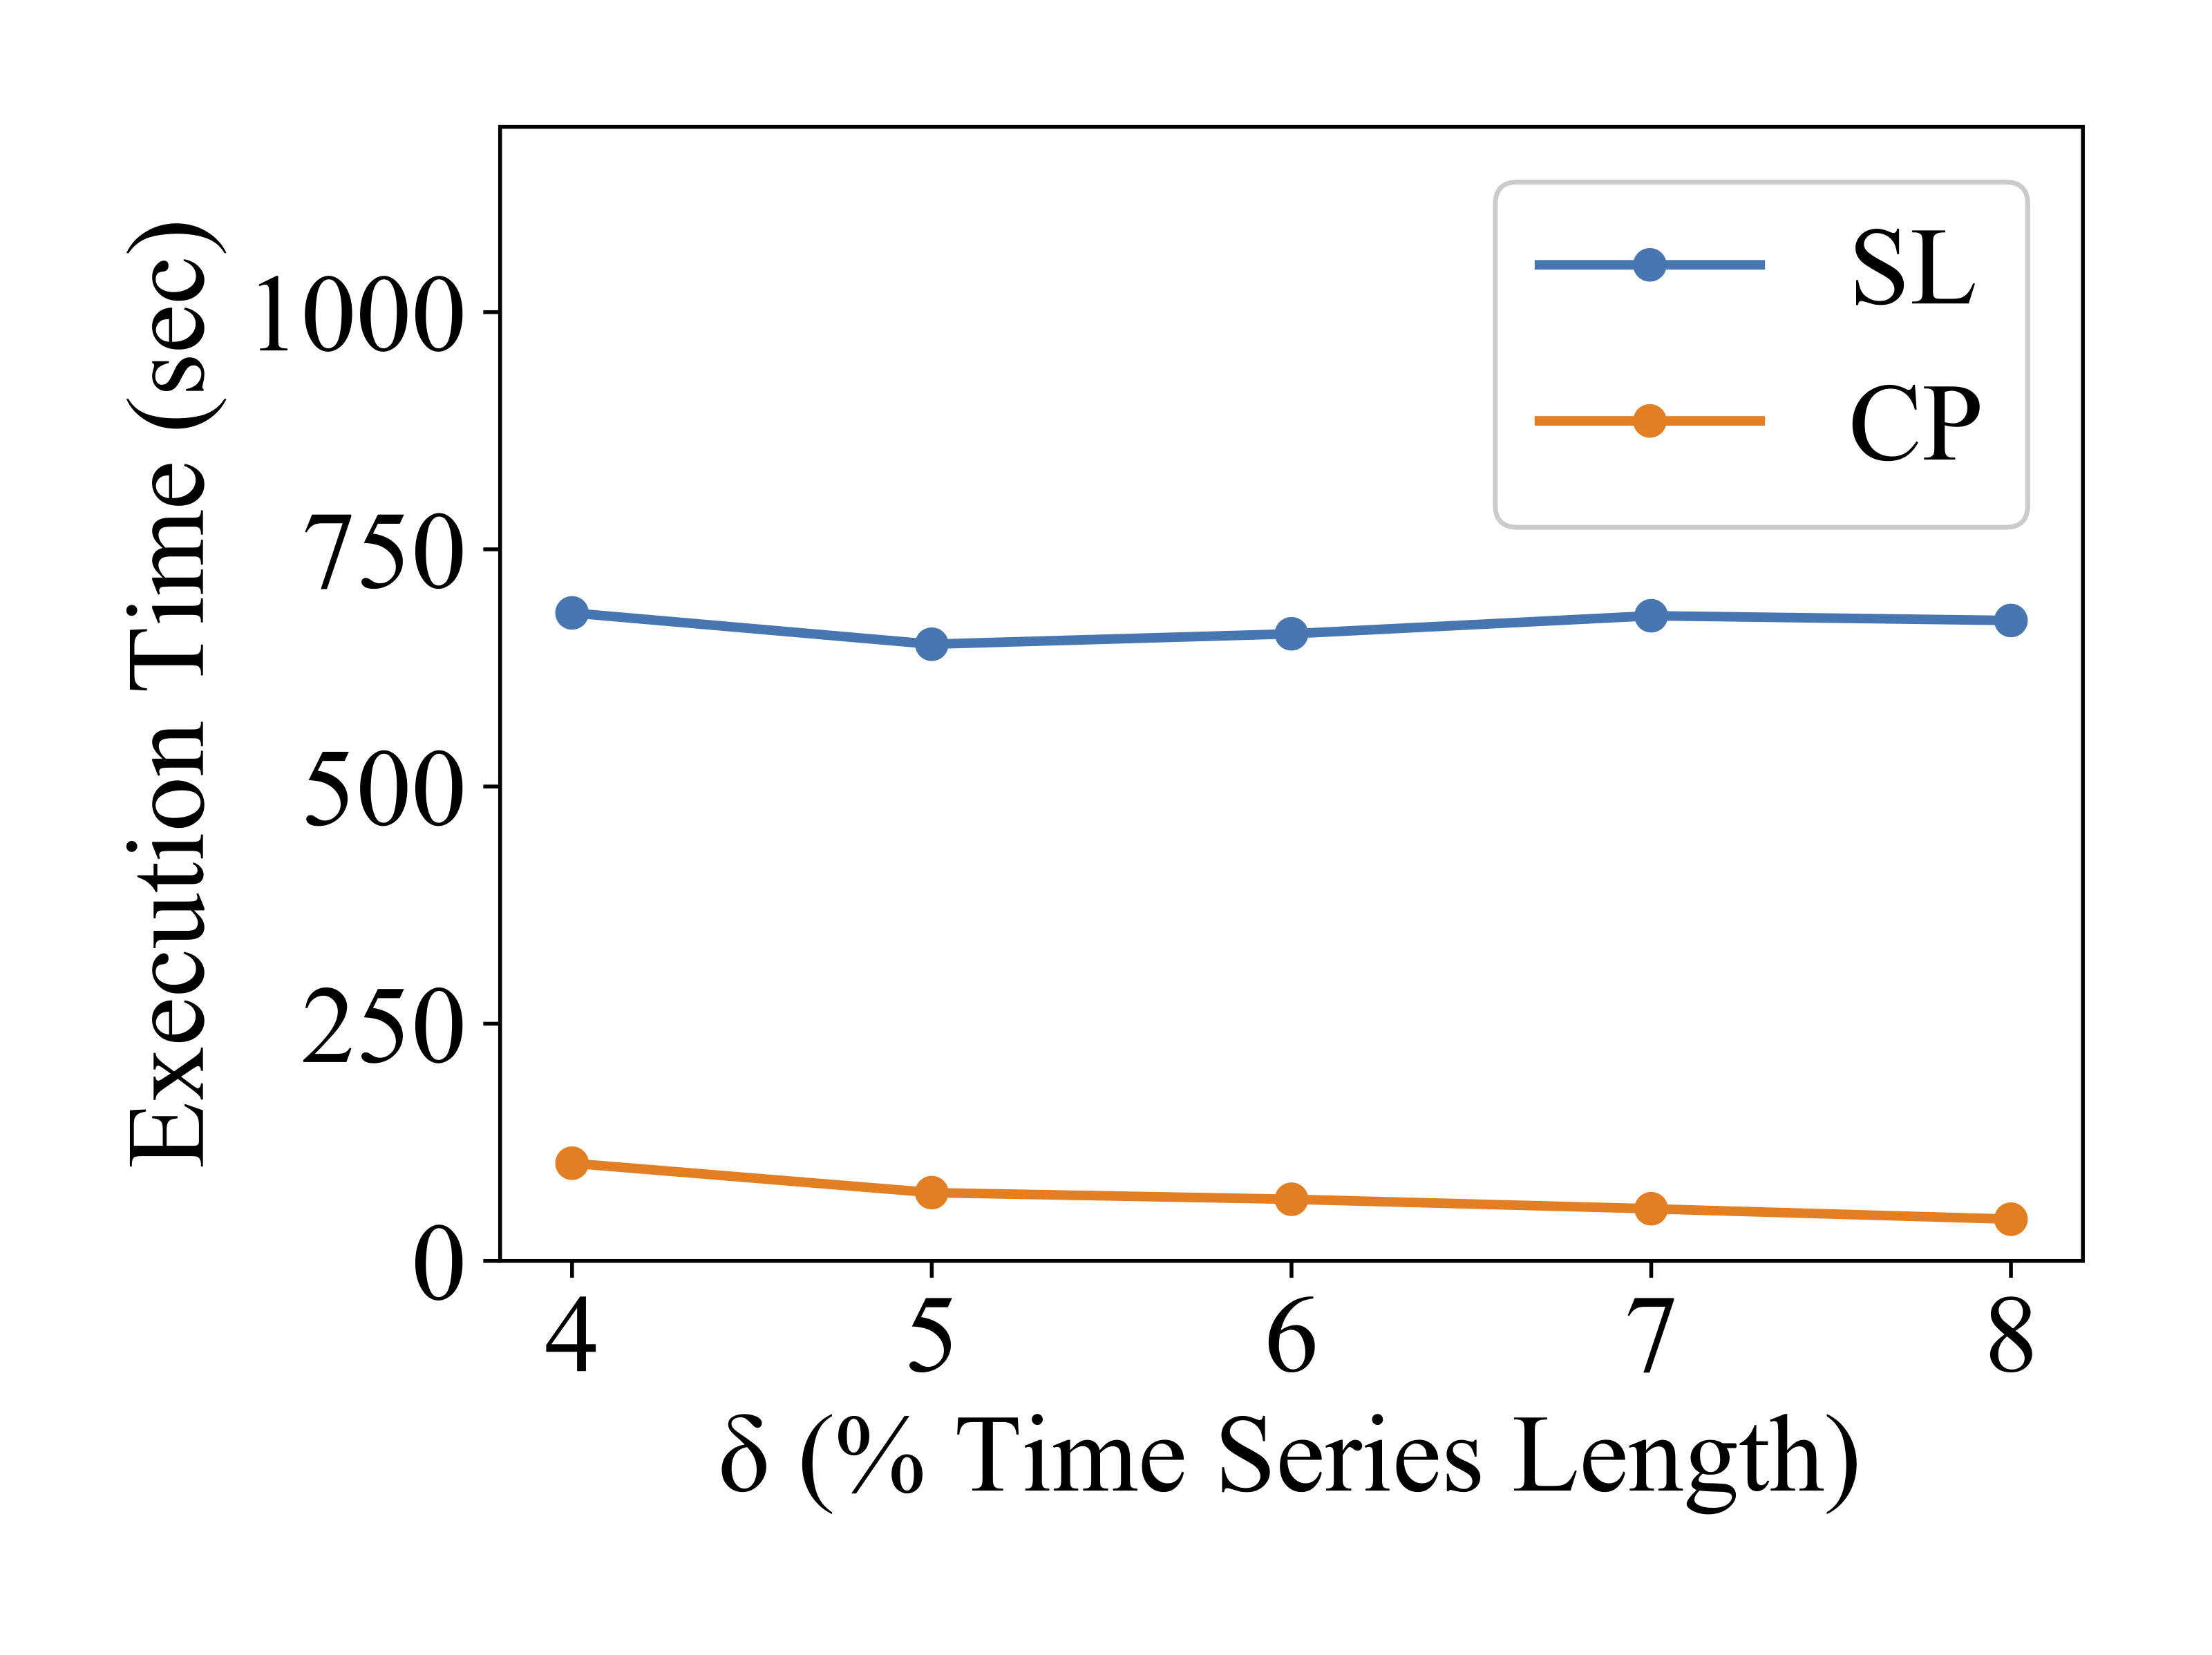
\includegraphics[trim=0.5cm 0.5cm 0.5cm 0.5cm, clip, width=0.45\textwidth]{figures/plots/bundles/varying_delta.png}\label{subfig:var_delta}}
 \subfloat[Bundle discovery results]{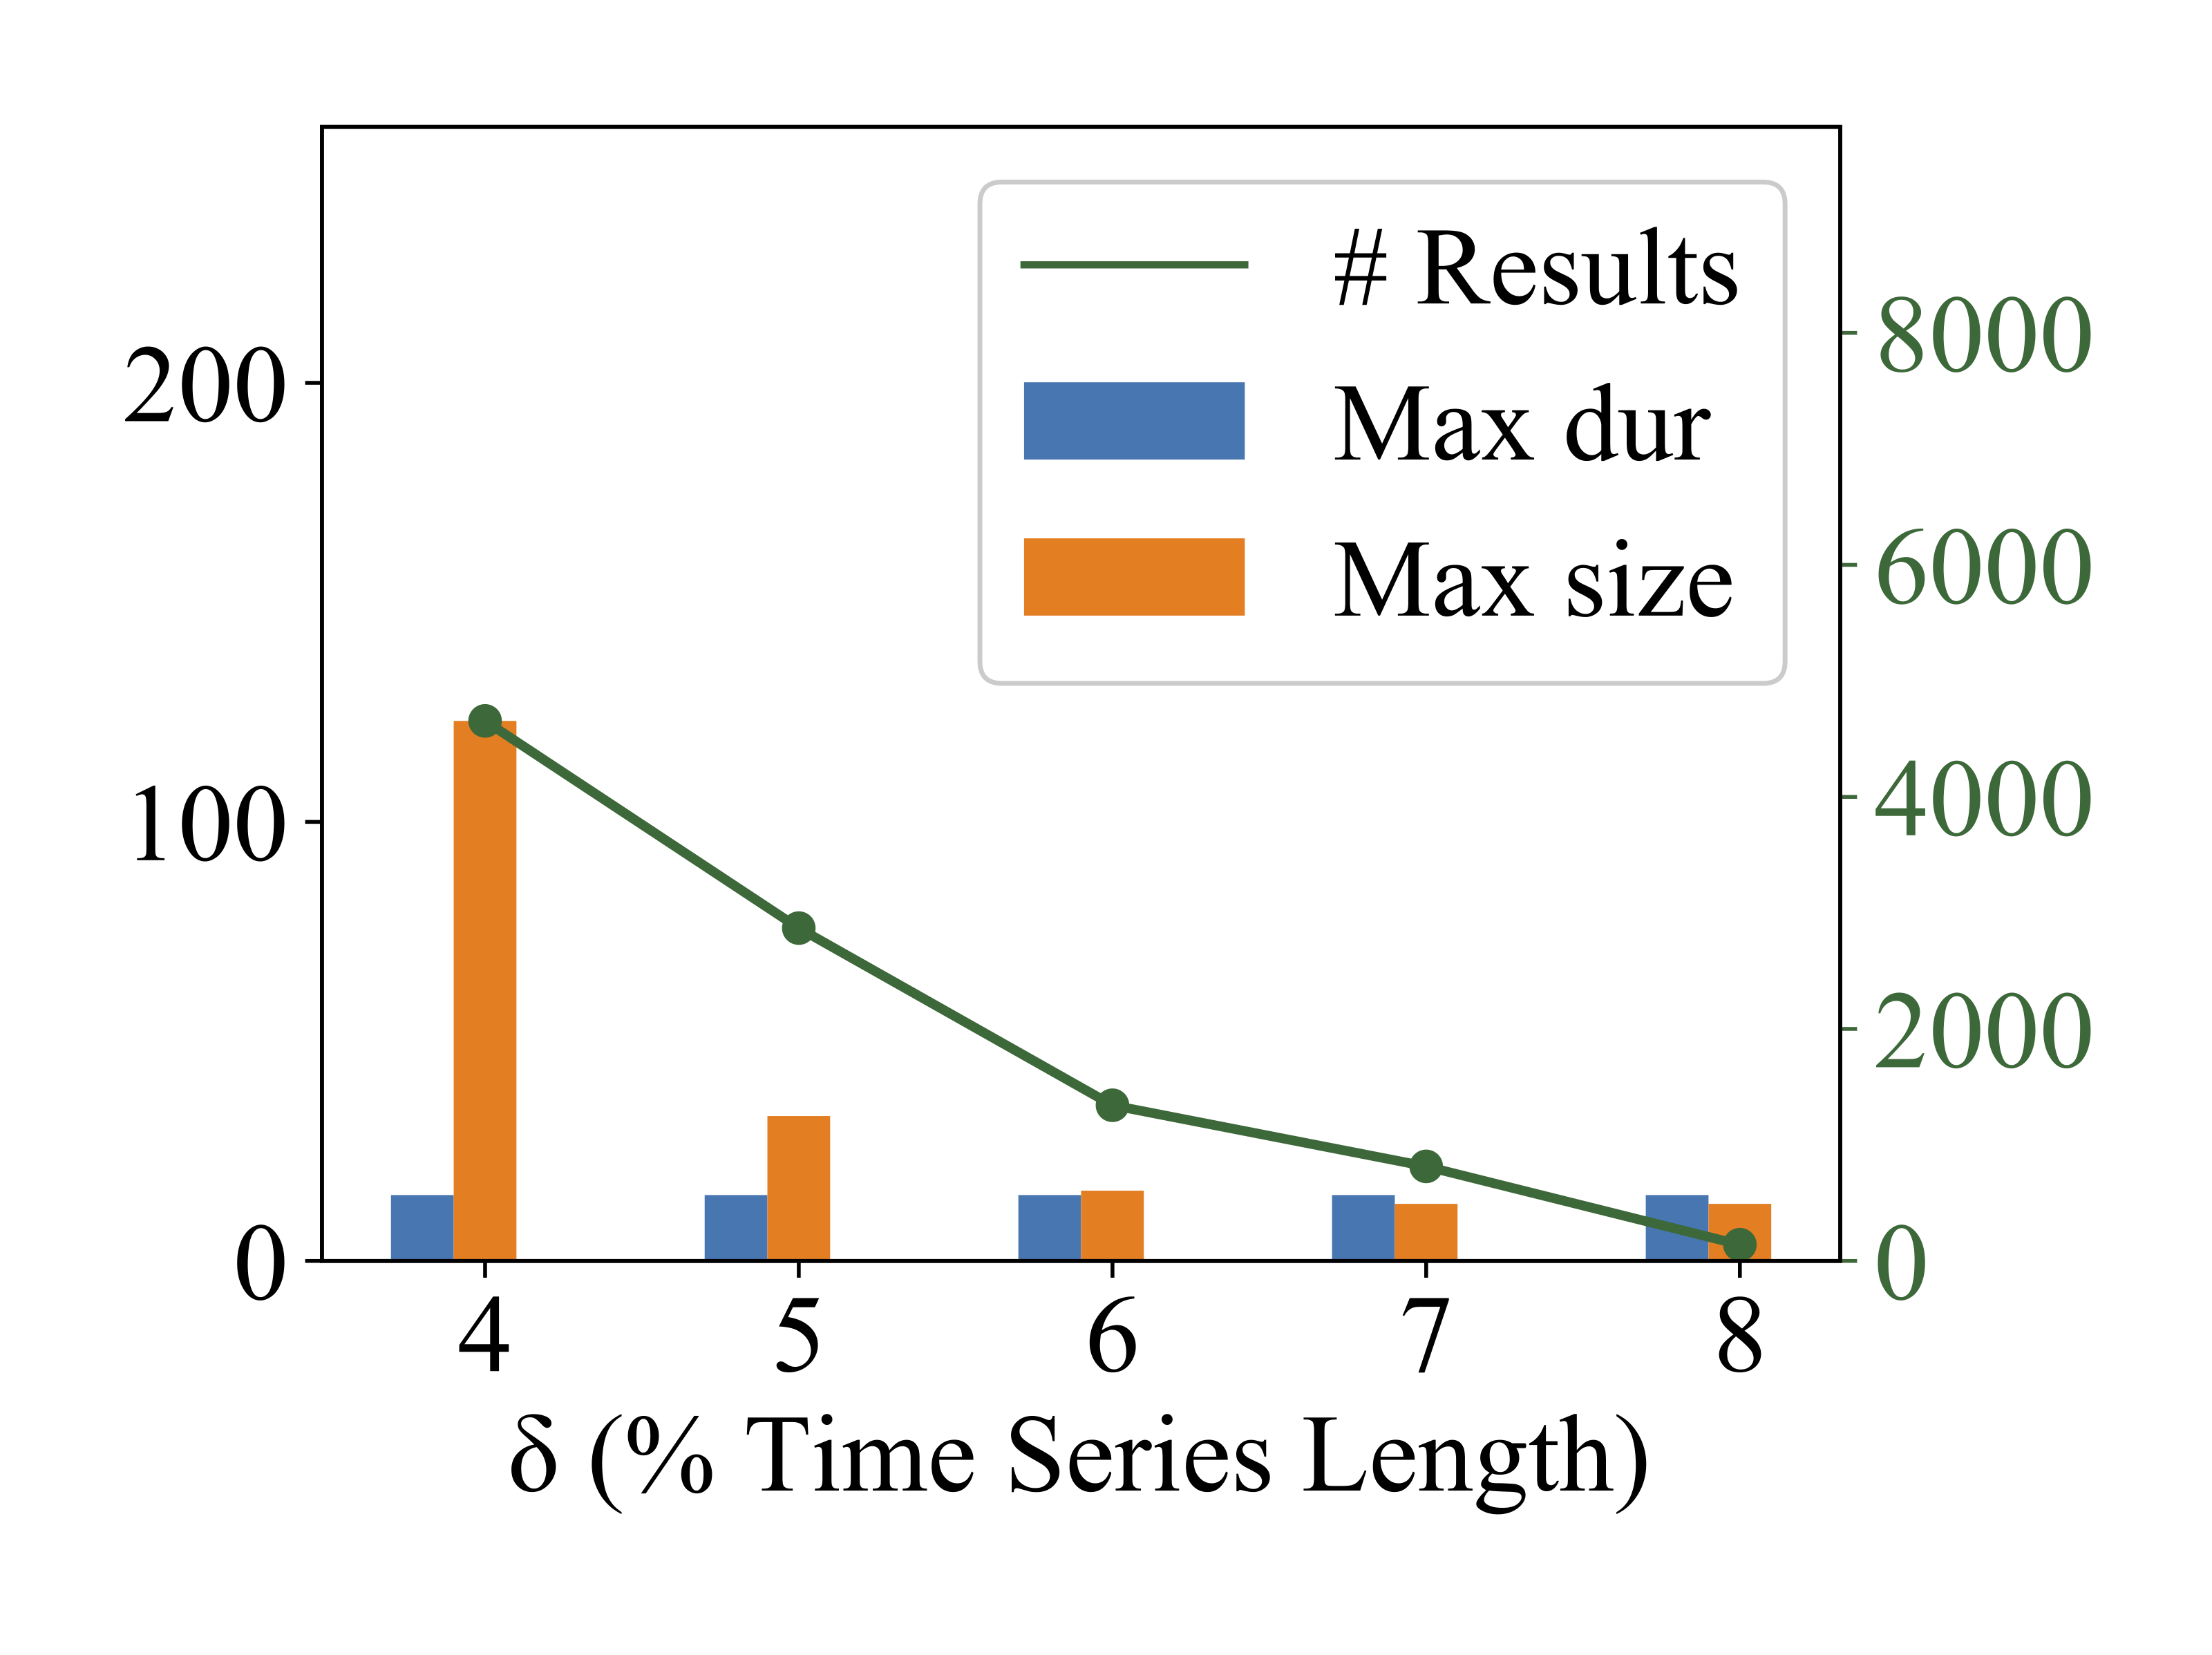
\includegraphics[trim=0.5cm 0.5cm 0.5cm 0.5cm, clip,width=0.45\textwidth]{figures/plots/bundles/varying_delta_bars.png}\label{subfig:var_delta_bars}} \\
 \subfloat[Pair discovery execution time]{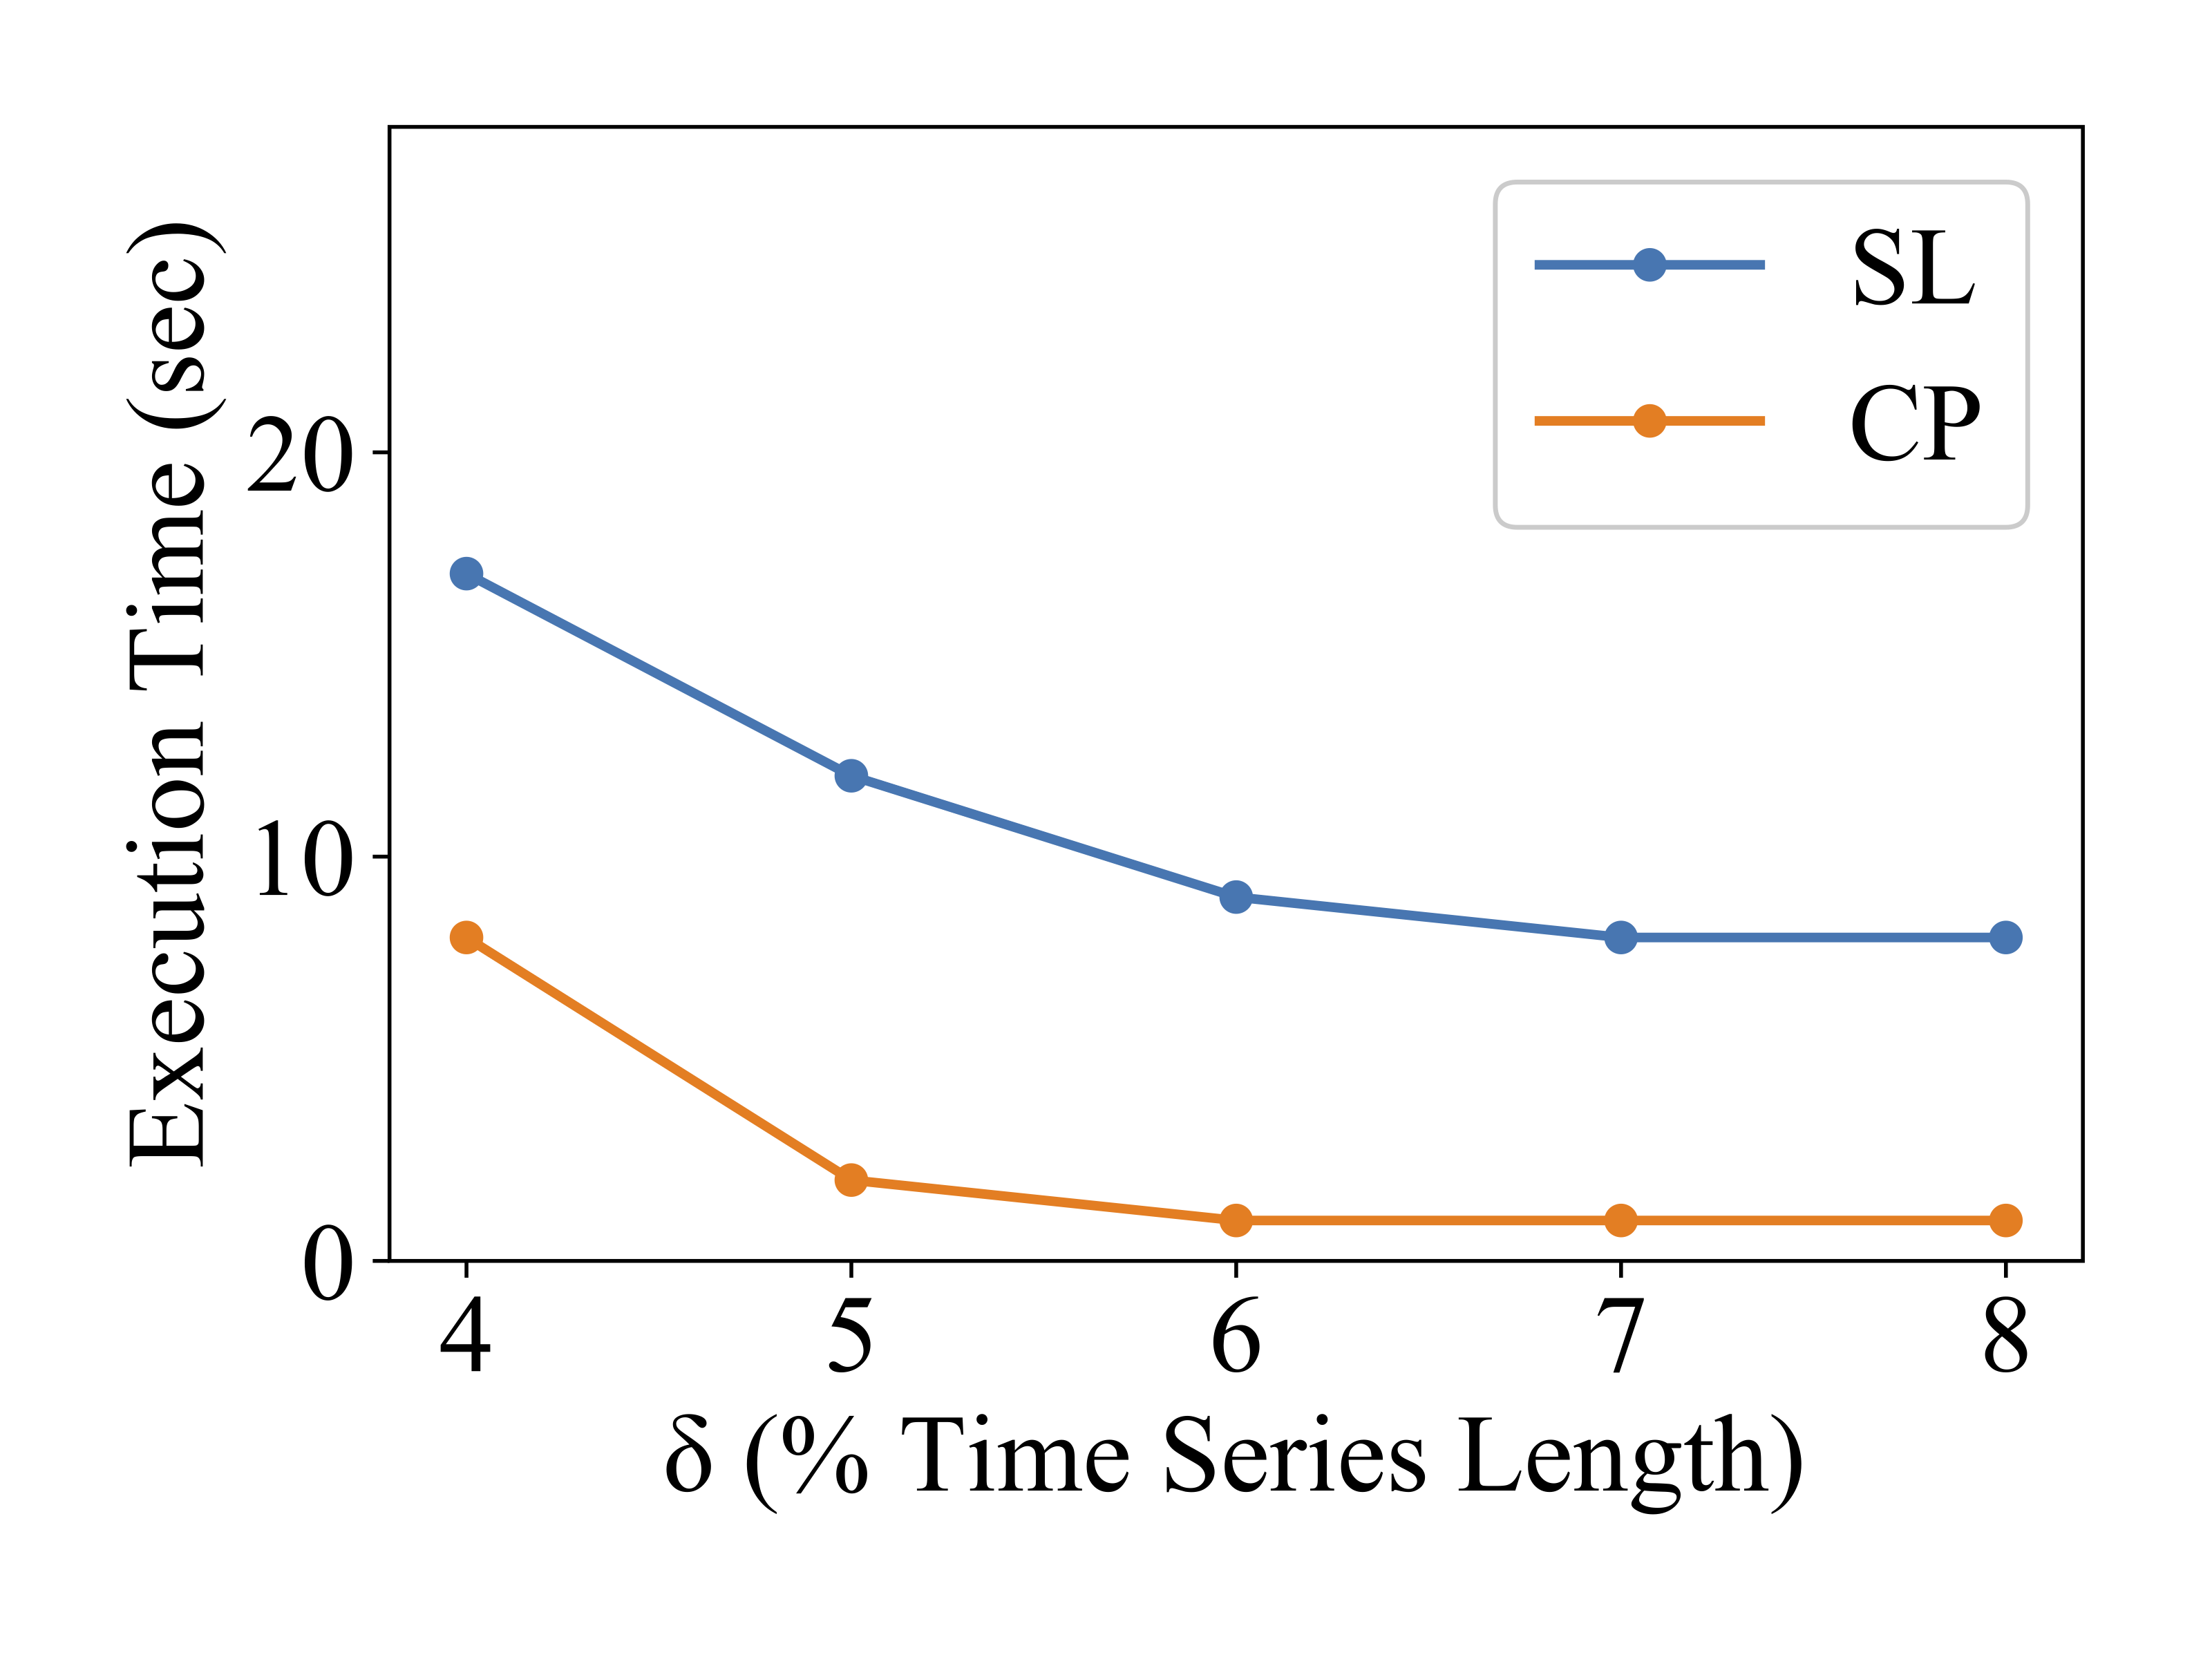
\includegraphics[trim=0.5cm 0.5cm 0.5cm 0.5cm, clip,width=0.45\textwidth]{figures/plots/pairs/varying_delta.png}\label{subfig:var_delta_bars_pairs}}
 \subfloat[Pair Discovery results]{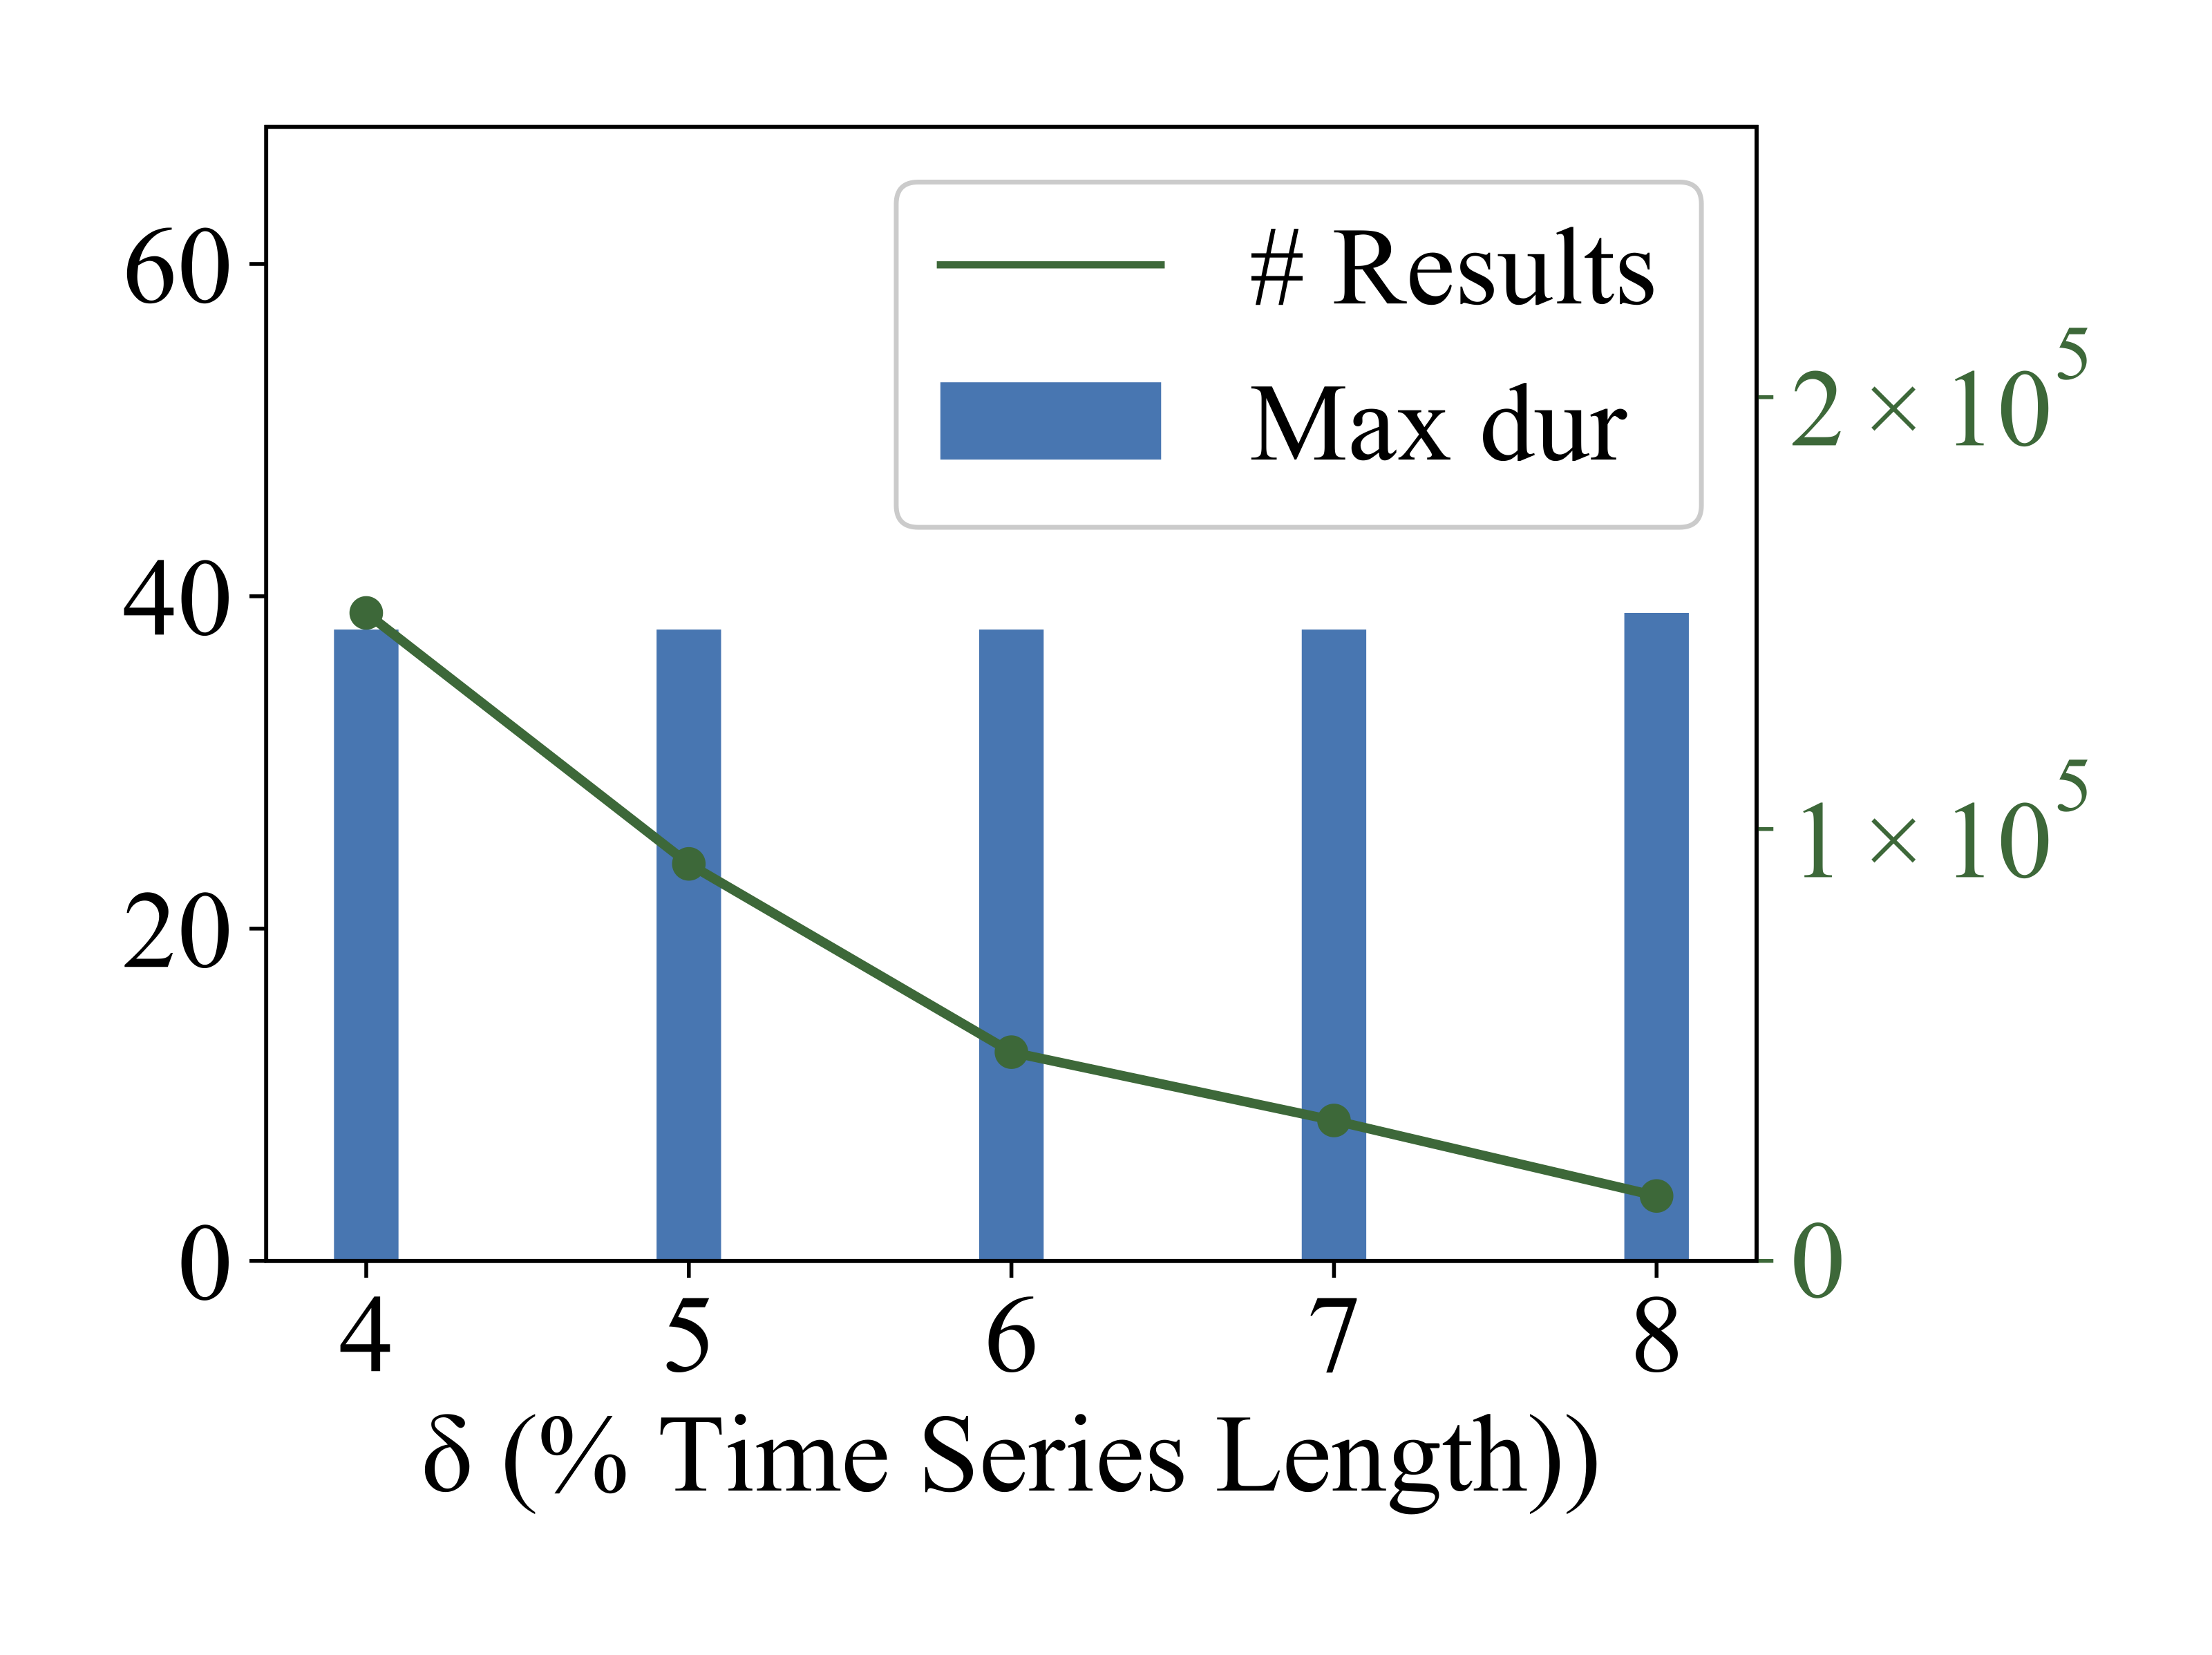
\includegraphics[trim=0.5cm 0.5cm 0.5cm 0.5cm, clip,width=0.45\textwidth]{figures/plots/pairs/varying_delta_bars.png}\label{subfig:var_delta_bars_pairs_bars}}
 \caption{Assessment against real data for varying $\delta$.}
 \label{fig:exp1}
\end{figure}

Figure \ref{fig:exp1} depicts the results for varying minimal duration $\delta$. In bundle discovery, the CP algorithm outperforms SL up to an order of magnitude in terms of execution time (Figure \ref{subfig:var_delta}). As the threshold $\delta$ gets larger, performance is improved due to less checkpoints being specified and less candidates needing verification. On the contrary, the SL approach performs similarly irrespective of $\delta$, as time series must be checked at all timestamps. From Figure \ref{subfig:var_delta_bars}, it turns out that the number of detected bundles is reduced as the $\delta$ value increases, which is expected as fewer bundles can last longer. In this plot, the blue bars indicate the maximum bundle duration among the ones that were detected, while the orange bars indicate the larger detected bundle in terms of membership. It is clear that the maximum bundle size is drastically reduced as the number of results diminish, while the maximum duration among bundles remains the same with the increase of $\delta$, as the longest bundle is the same in these results.

Regarding pair discovery, since it is an overall faster process, the differences in terms of efficiency are smaller, but still apparent. In this case, the execution time (Figure \ref{subfig:var_delta_bars_pairs}) is more abruptly reduced in both SL and CP methods, since less subsequences qualify as pairs. The number of results (Figure \ref{subfig:var_delta_bars_pairs_bars}) is now naturally much larger, as far more pairs are expected to be verified if bundles exist. The same stands for the maximum duration among pairs, which tend to last longer compared to bundles. Since a pair is actually a bundle with $\mu$=2 members, it is easier to find local similarity over longer intervals between two subsequences rather than an increased number of them. The maximum duration, as in bundle discovery, remains the same as $\delta$ increases, since this corresponds to the same pair in the results. 

\paragraph{Varying $\epsilon$}
\begin{figure}[!ht]
 \centering
 \subfloat[Bundle discovery execution time]{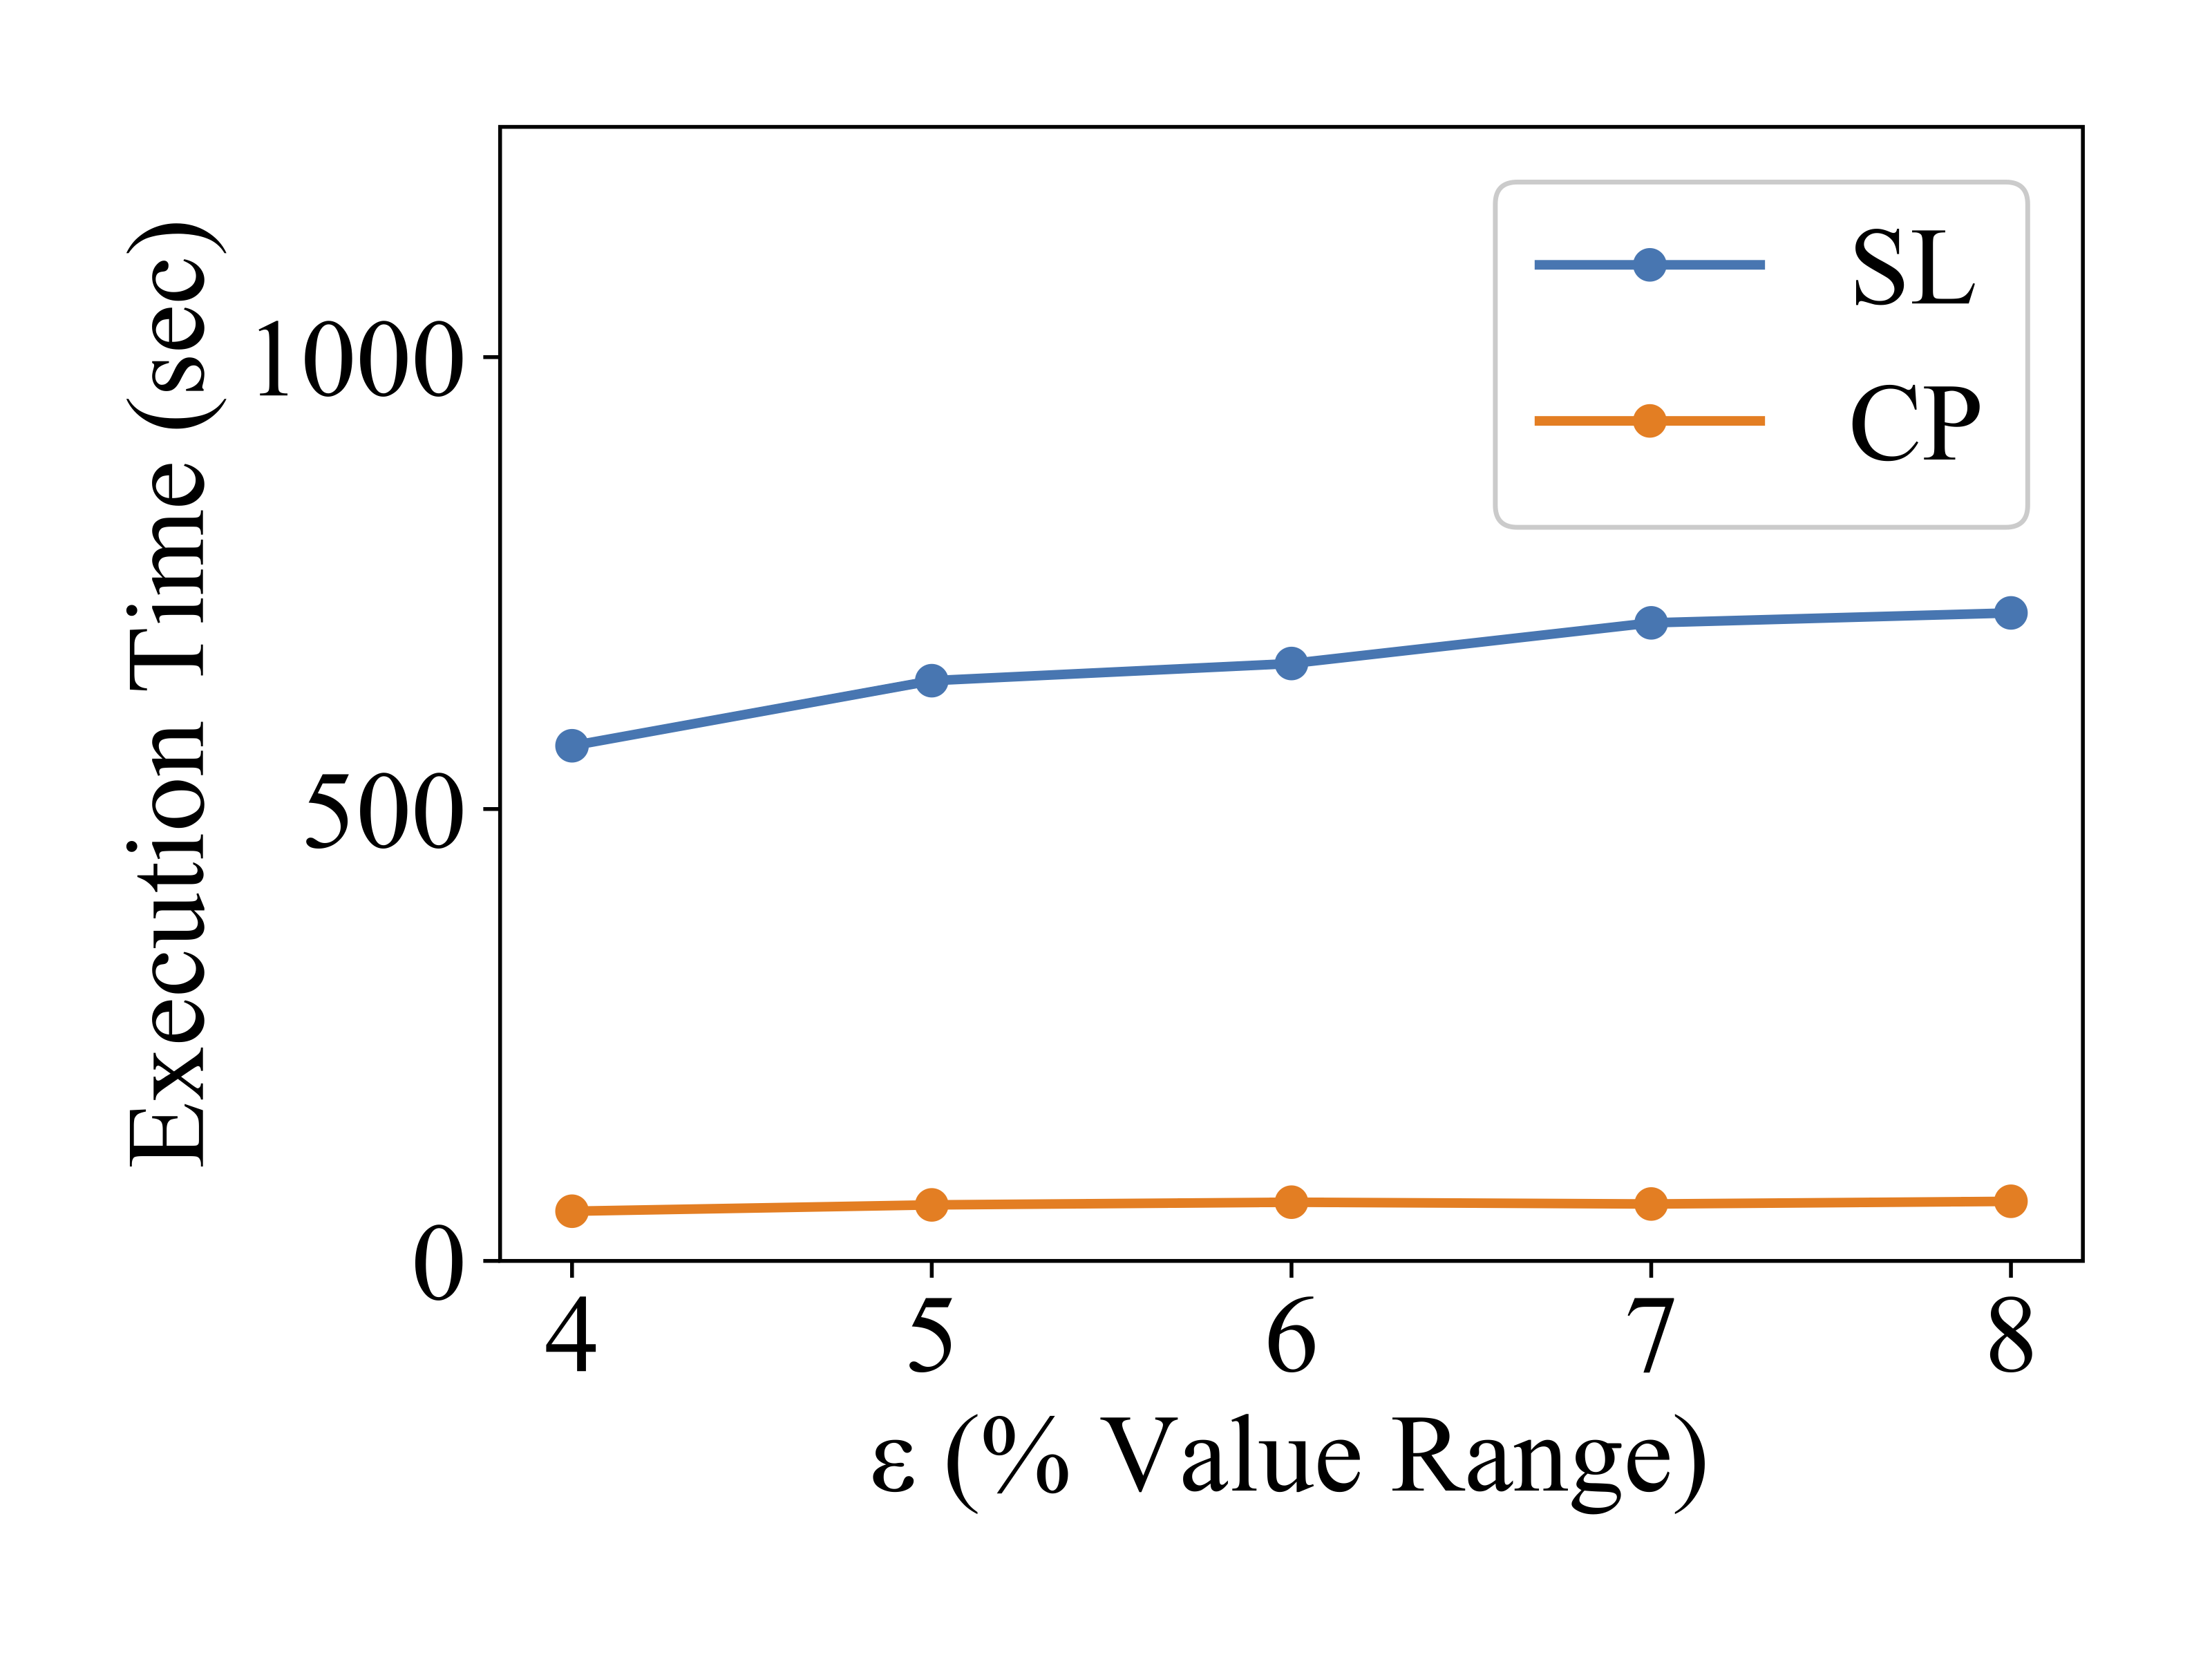
\includegraphics[trim=0.5cm 0.5cm 0.5cm 0.5cm, clip,width=0.45\textwidth]{figures/plots/bundles/varying_epsilon.png}\label{subfig:var_eps}}
 \subfloat[Bundle discovery results]{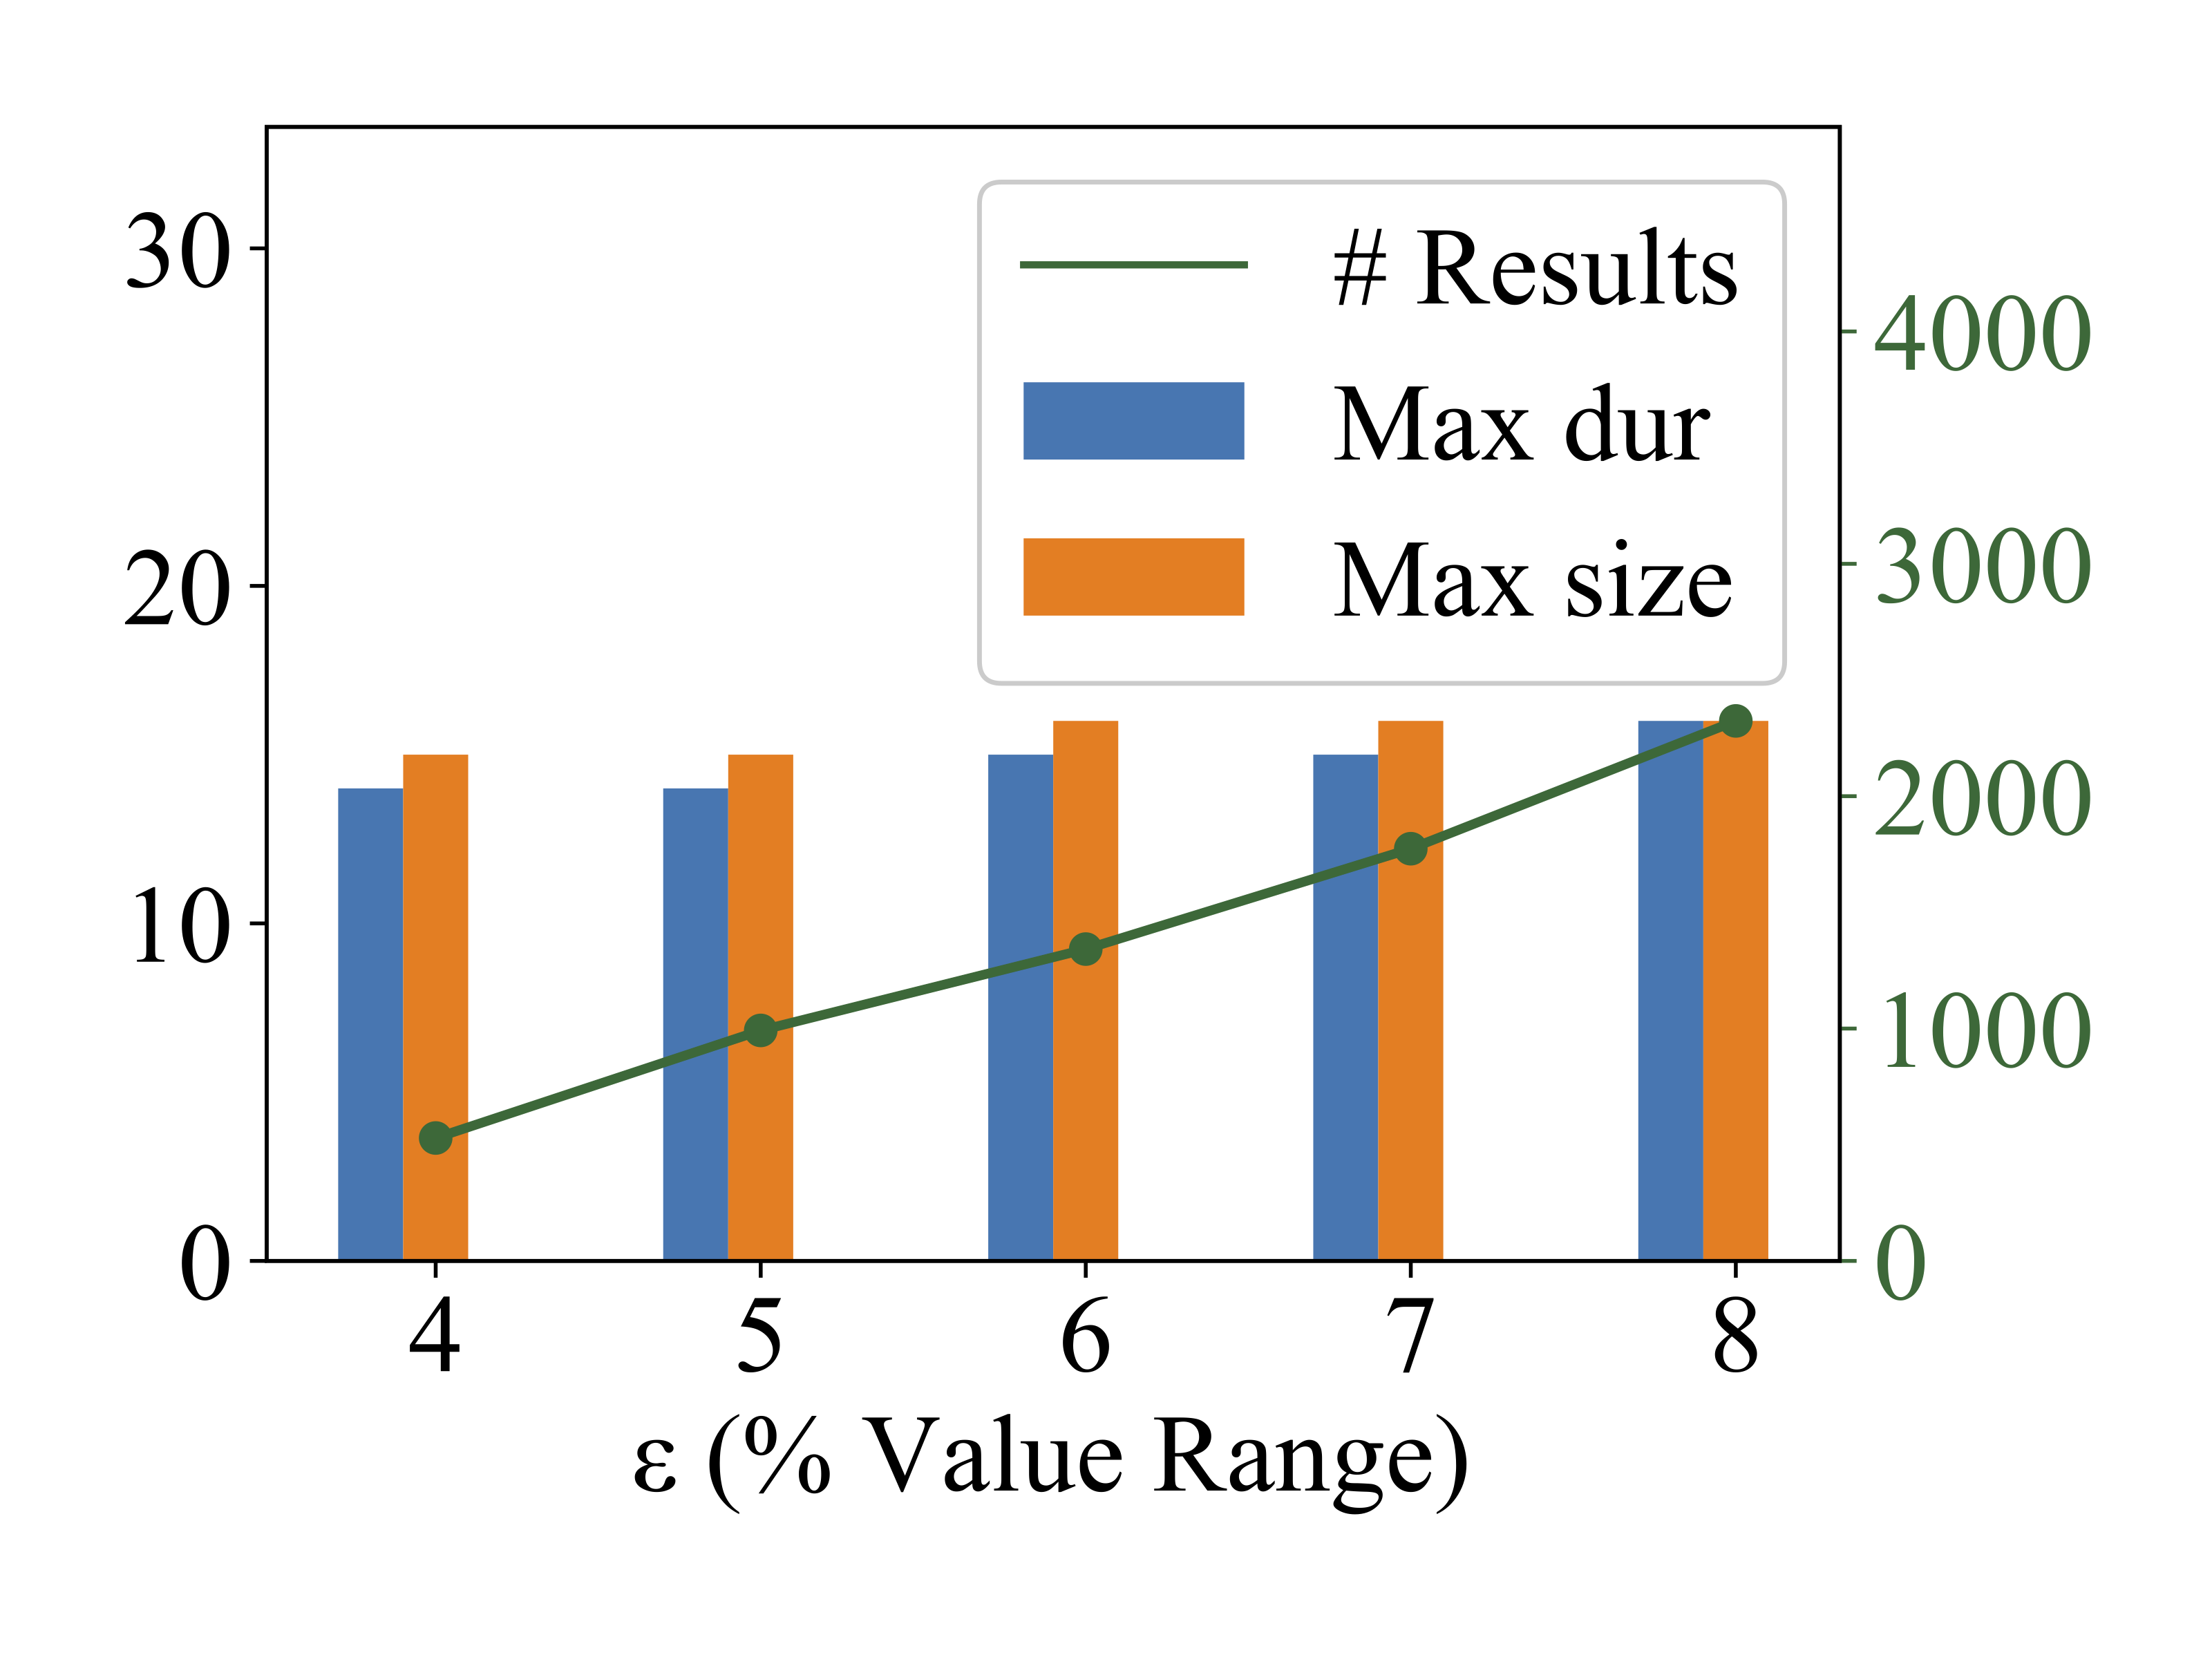
\includegraphics[trim=0.5cm 0.5cm 0.5cm 0.5cm, clip,width=0.45\textwidth]{figures/plots/bundles/varying_epsilon_bars.png}\label{subfig:var_eps_bars}} \\
 \subfloat[Pair discovery execution time]{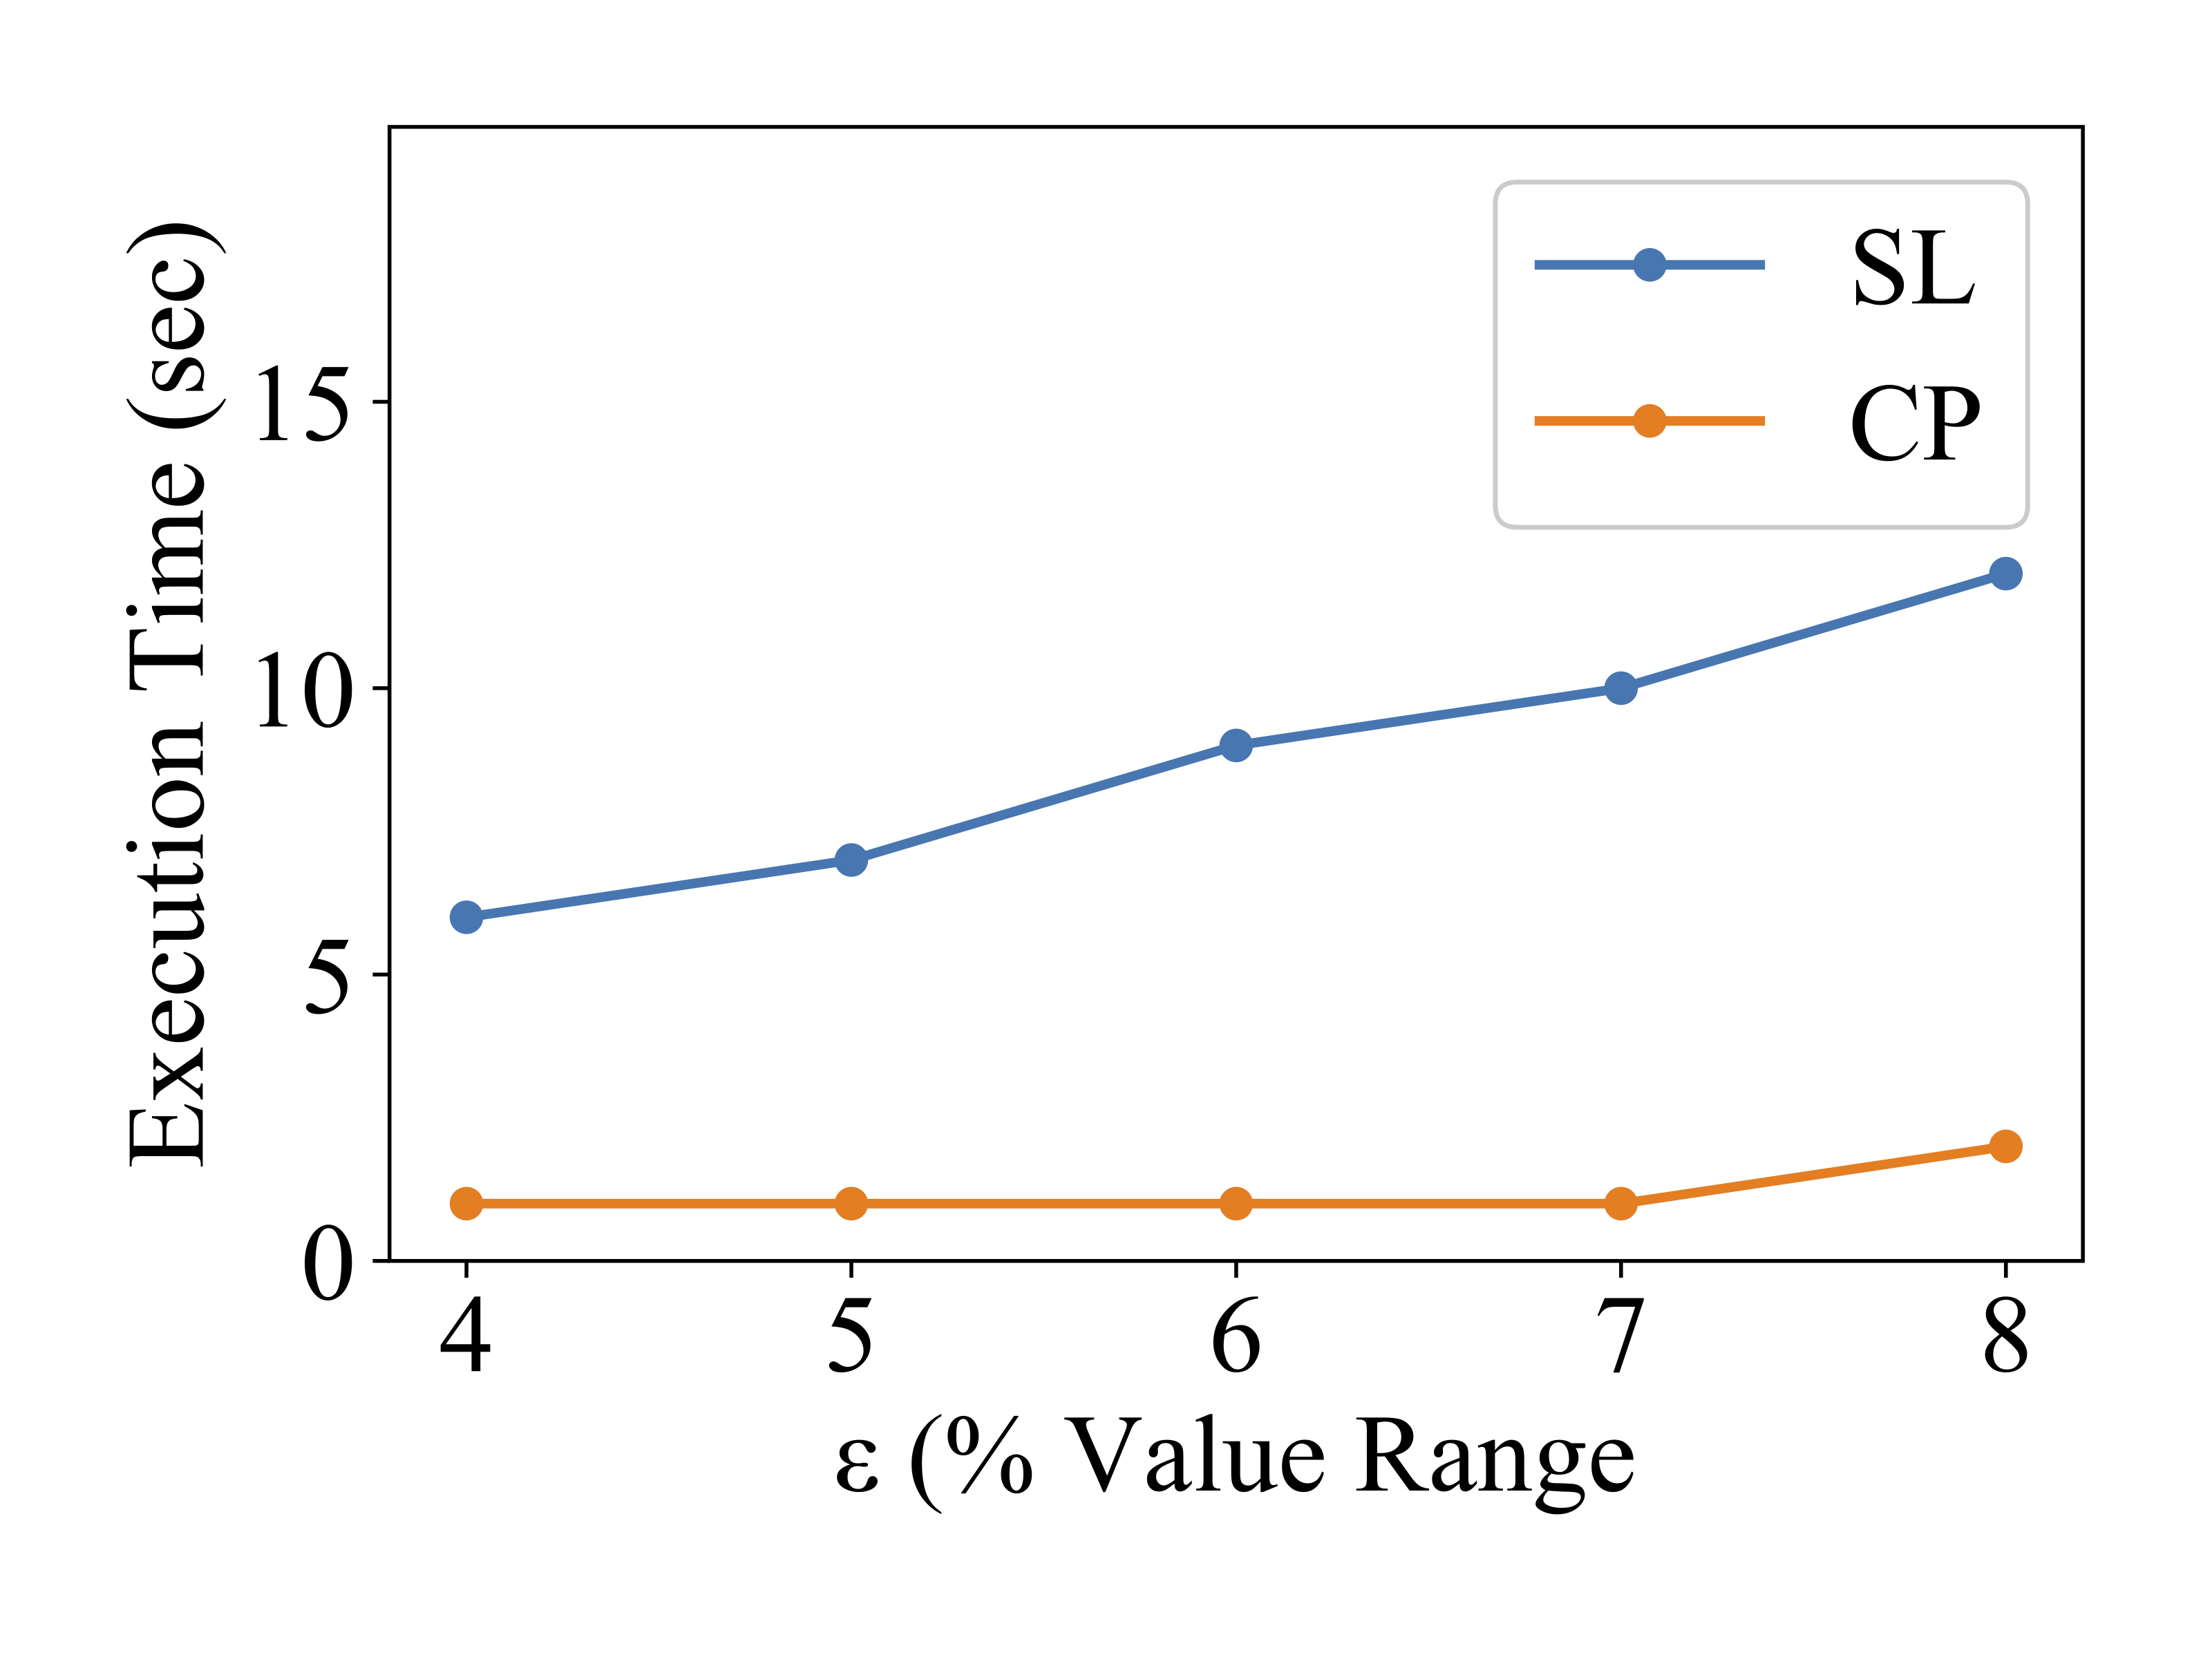
\includegraphics[trim=0.5cm 0.5cm 0.5cm 0.5cm, clip,width=0.45\textwidth]{figures/plots/pairs/varying_epsilon.png}\label{subfig:var_eps_bars_pairs}}
 \subfloat[Pair Discovery results]{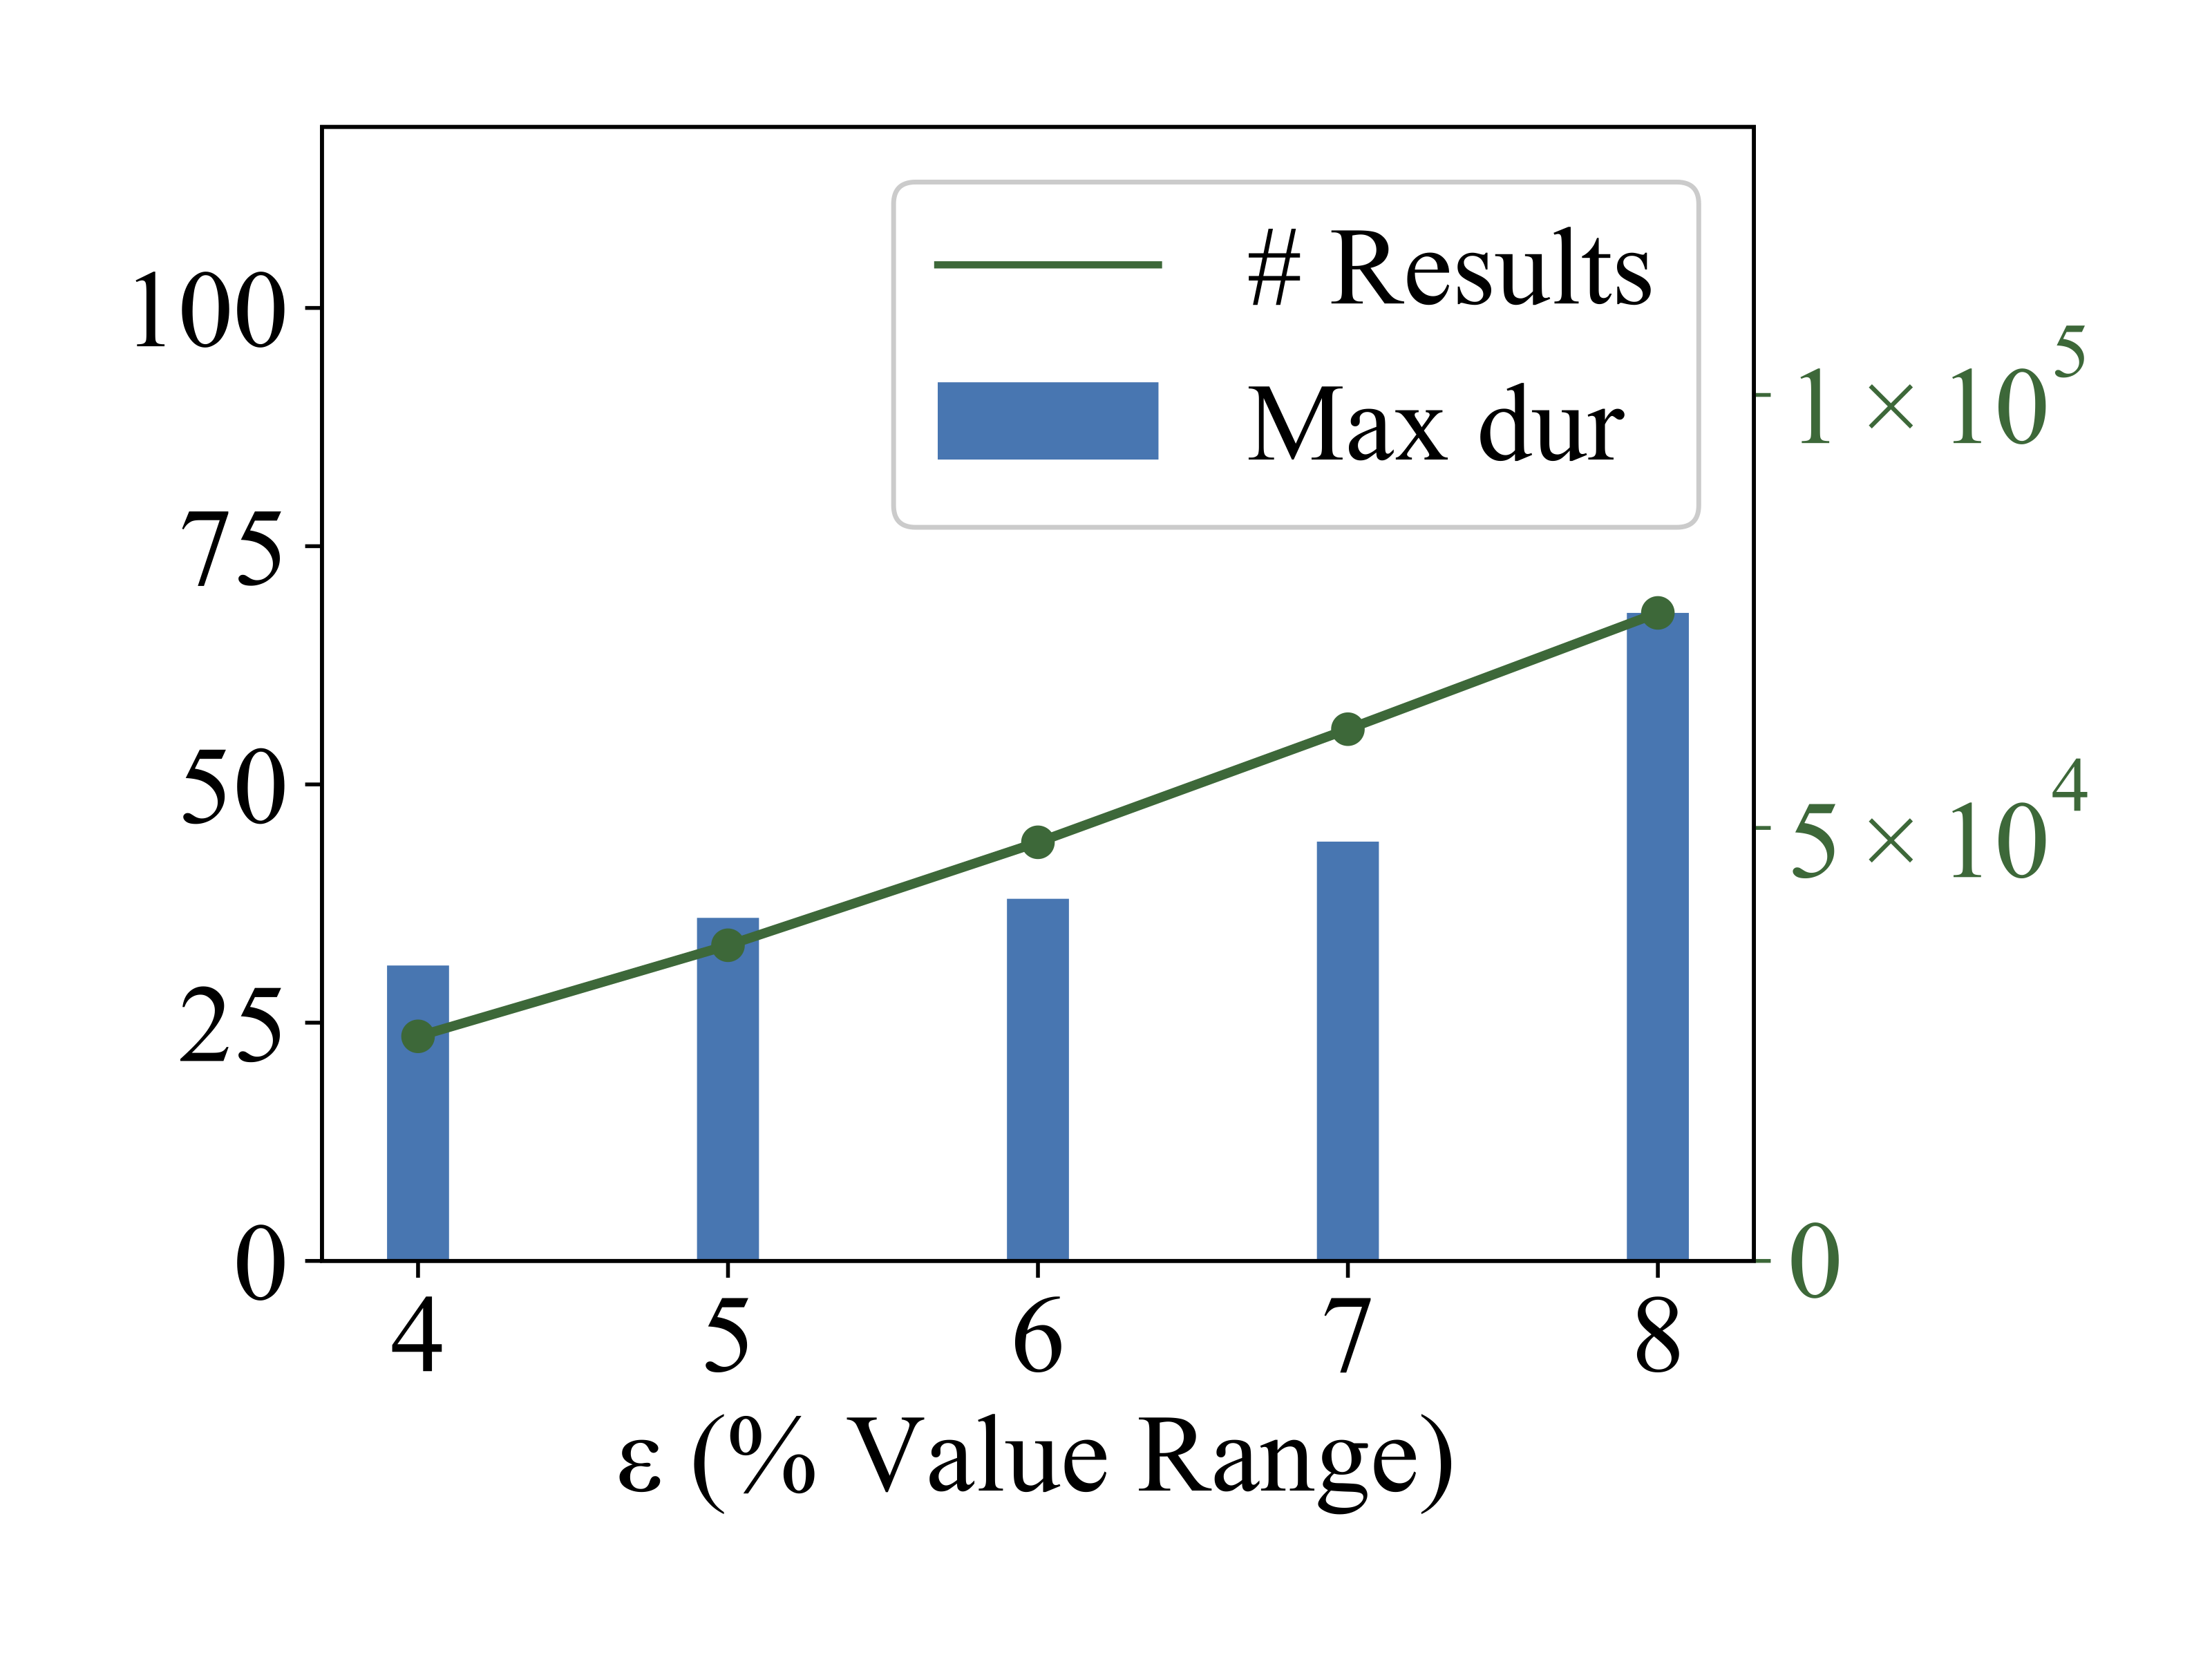
\includegraphics[trim=0.5cm 0.5cm 0.5cm 0.5cm, clip,width=0.45\textwidth]{figures/plots/pairs/varying_epsilon_bars.png}\label{subfig:var_eps_bars_pairs_bars}}
 \caption{Assessment against real data for varying $\epsilon$.}
 \label{fig:exp2}
\end{figure}

Varying threshold $\epsilon$ for bundle discovery slightly incurs more execution cost for both SL and CP approaches. This is due to the increased number of bundles that need to be verified. Nonetheless, the difference in cost remains at levels of at most an order of magnitude, as shown in Figure \ref{subfig:var_eps}. As expected, the number of results is also increased (Figure \ref{subfig:var_eps_bars}. So does the maximum duration bundle, which is also expected due to more qualifying bundles, hence a higher probability to find longer ones. The maximum bundle size (i.e., membership) is also increased, as more time series can form a bundle when allowing a wider threshold $\epsilon$ in deviation of their respective values.

Regarding pair discovery, the results are again similar to bundle discovery for varying $\epsilon$. For very small $\epsilon$ values of up to 7\% of the value range, the CP algorithm returns results almost instantly. The SL approach is at least five times slower, with its performance deteriorating more rapidly with increasing $\epsilon$ values. Again, as in bundle discovery, the results are growing with greater $\epsilon$, as does the maximum duration among pairs, especially for $\epsilon$ equal to 8\% of the value range.

\paragraph{Varying $\mu$}
\begin{figure}[!ht]
 \centering
 \subfloat[Bundle discovery execution time]{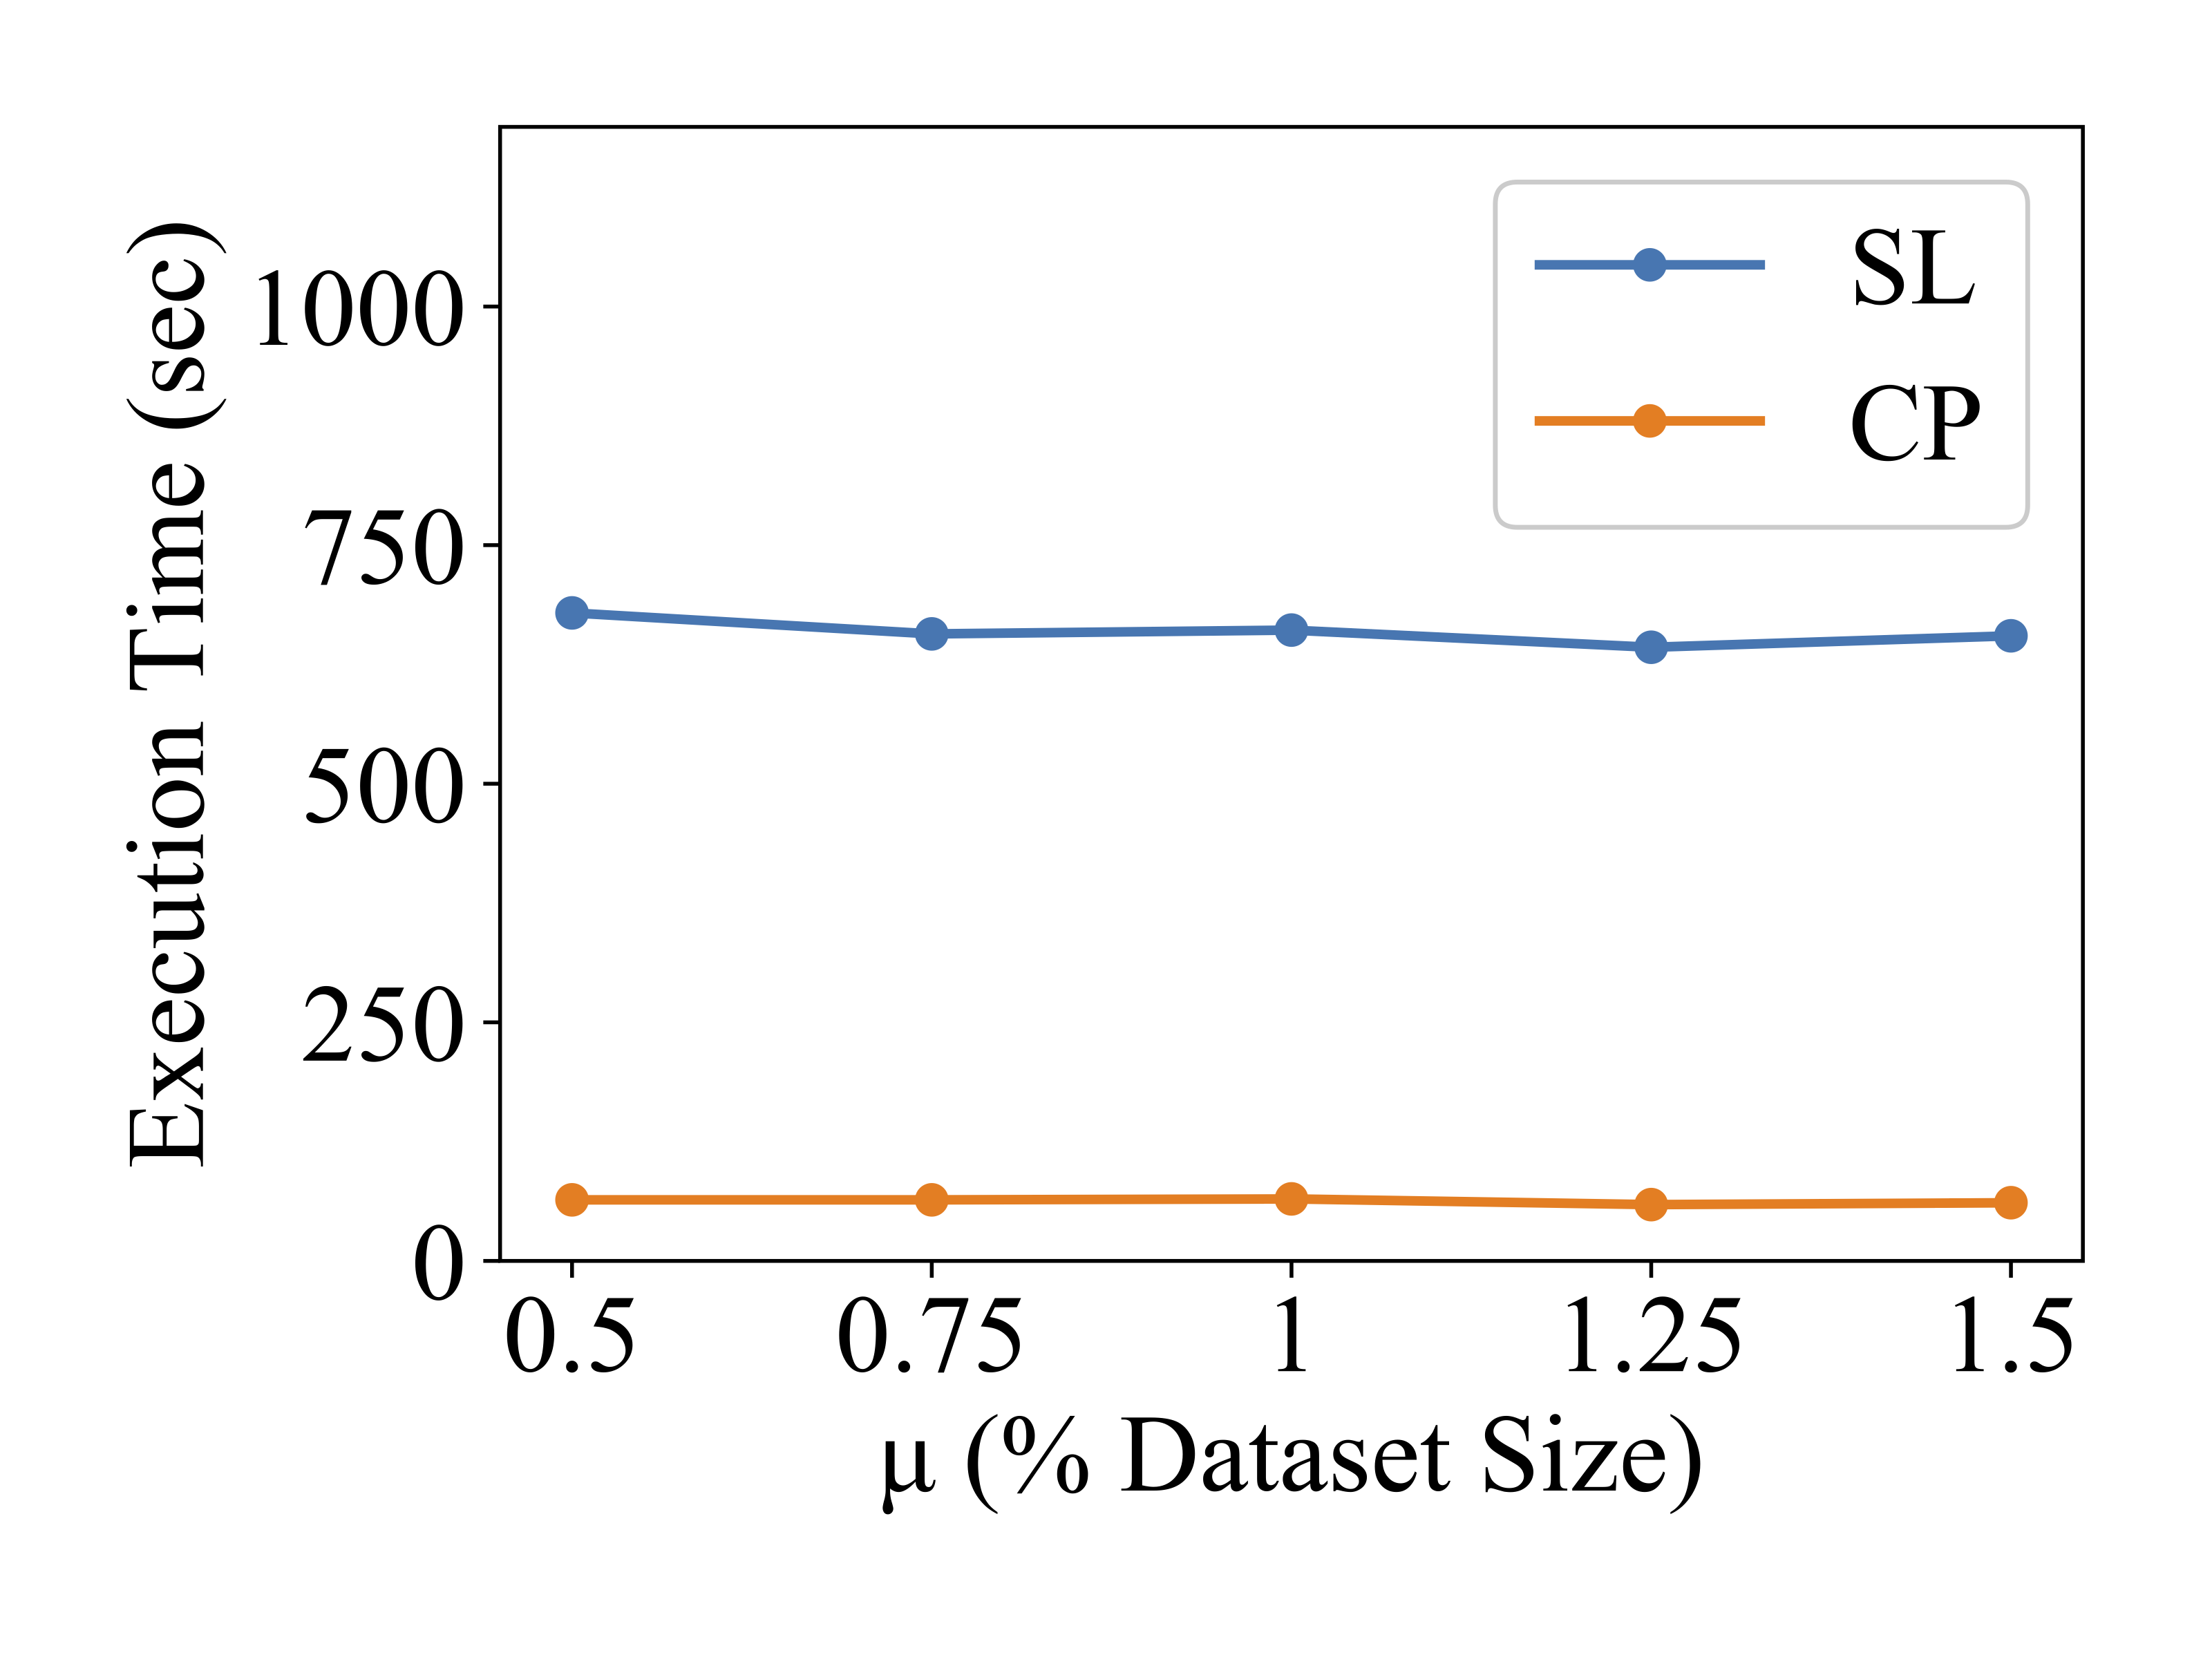
\includegraphics[trim=0.5cm 0.5cm 0.5cm 0.5cm, clip,width=0.45\textwidth]{figures/plots/bundles/varying_mu.png}\label{subfig:var_mu}}
 \subfloat[Bundle discovery results]{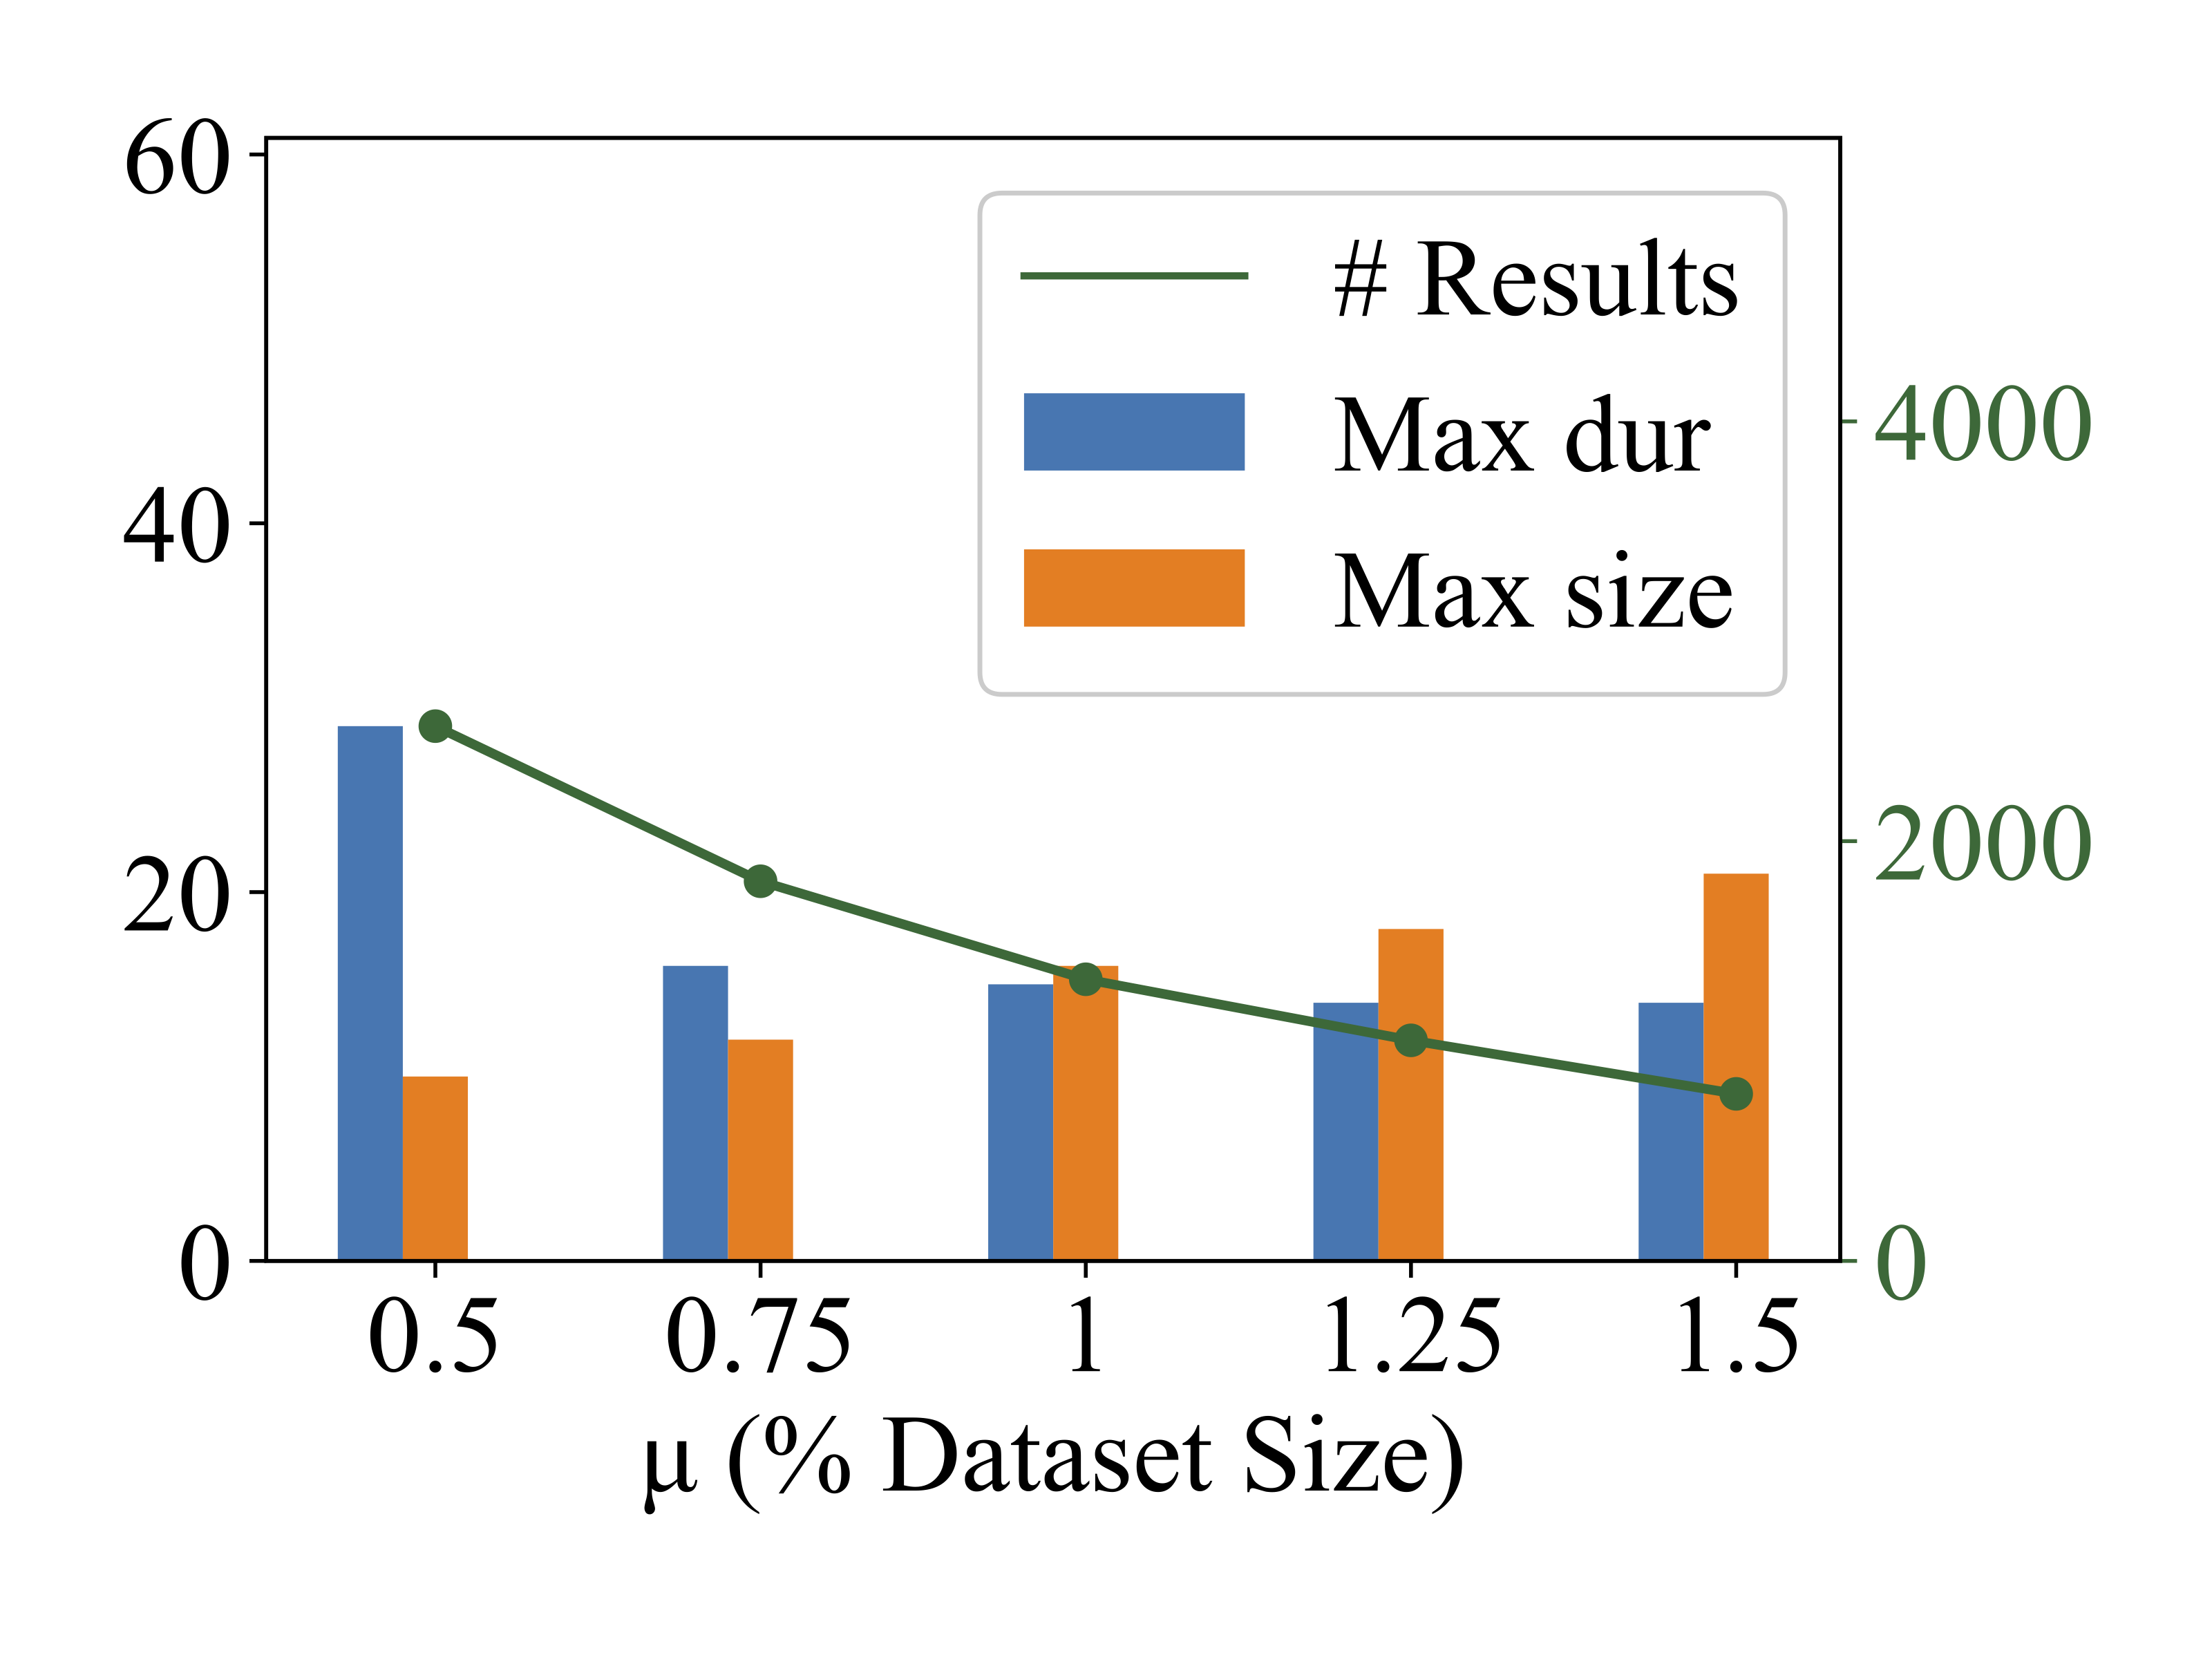
\includegraphics[trim=0.5cm 0.5cm 0.5cm 0.5cm, clip,width=0.45\textwidth]{figures/plots/bundles/varying_mu_bars.png}\label{subfig:var_mu_bars}}
 \caption{Assessment against real data for varying $\mu$.}
 \label{fig:exp3}
\end{figure}

When varying the minimum membership parameter $\mu$ in bundle discovery (Figure \ref{fig:exp3}), the results regarding execution time are again very similar to the rest of the tests as indicated in Figure \ref{subfig:var_mu}. Again, the CP algorithm outperforms SL up to one order of magnitude. The execution time is very slightly decreased for larger $\mu$ values in both algorithms, as more candidate bundles are pruned. Results from CP are reported almost instantly, since the number of time series is rather small and scanning through the limited number of checkpoints is very fast. This explains why performance of SL does not get drastically improved as $\mu$ gets larger, since filtering and verification has to be repeated at every timestamp. The number of results (Figure~\ref{subfig:var_mu_bars}) is reduced as $\mu$ increases, which is expected, as less bundles get detected with a larger membership. The maximum duration among bundles also decreases; interestingly, the maximum size detected among bundles increases as the number of results diminishes, due to the growing number $\mu$ of required number of members per bundle.

\subsubsubsection{Efficiency against Synthetic Data}
\label{subsubsec:effic}
To evaluate the efficiency of our methods, we used the synthetic dataset. Regarding parameter values, as in the previous experiments, we performed preliminary tests to extract ranges of values where the algorithms return a reasonable number of results. Table \ref{tab:parameters2} lists the range of values for all parameters used in these efficiency tests for bundle and pair discovery, with the default values emphasized in bold (again, $\mu$ is not applicable in pair discovery).

\paragraph{Varying Dataset Size}
\begin{figure}[!ht]
 \centering
 \subfloat[Bundle discovery]{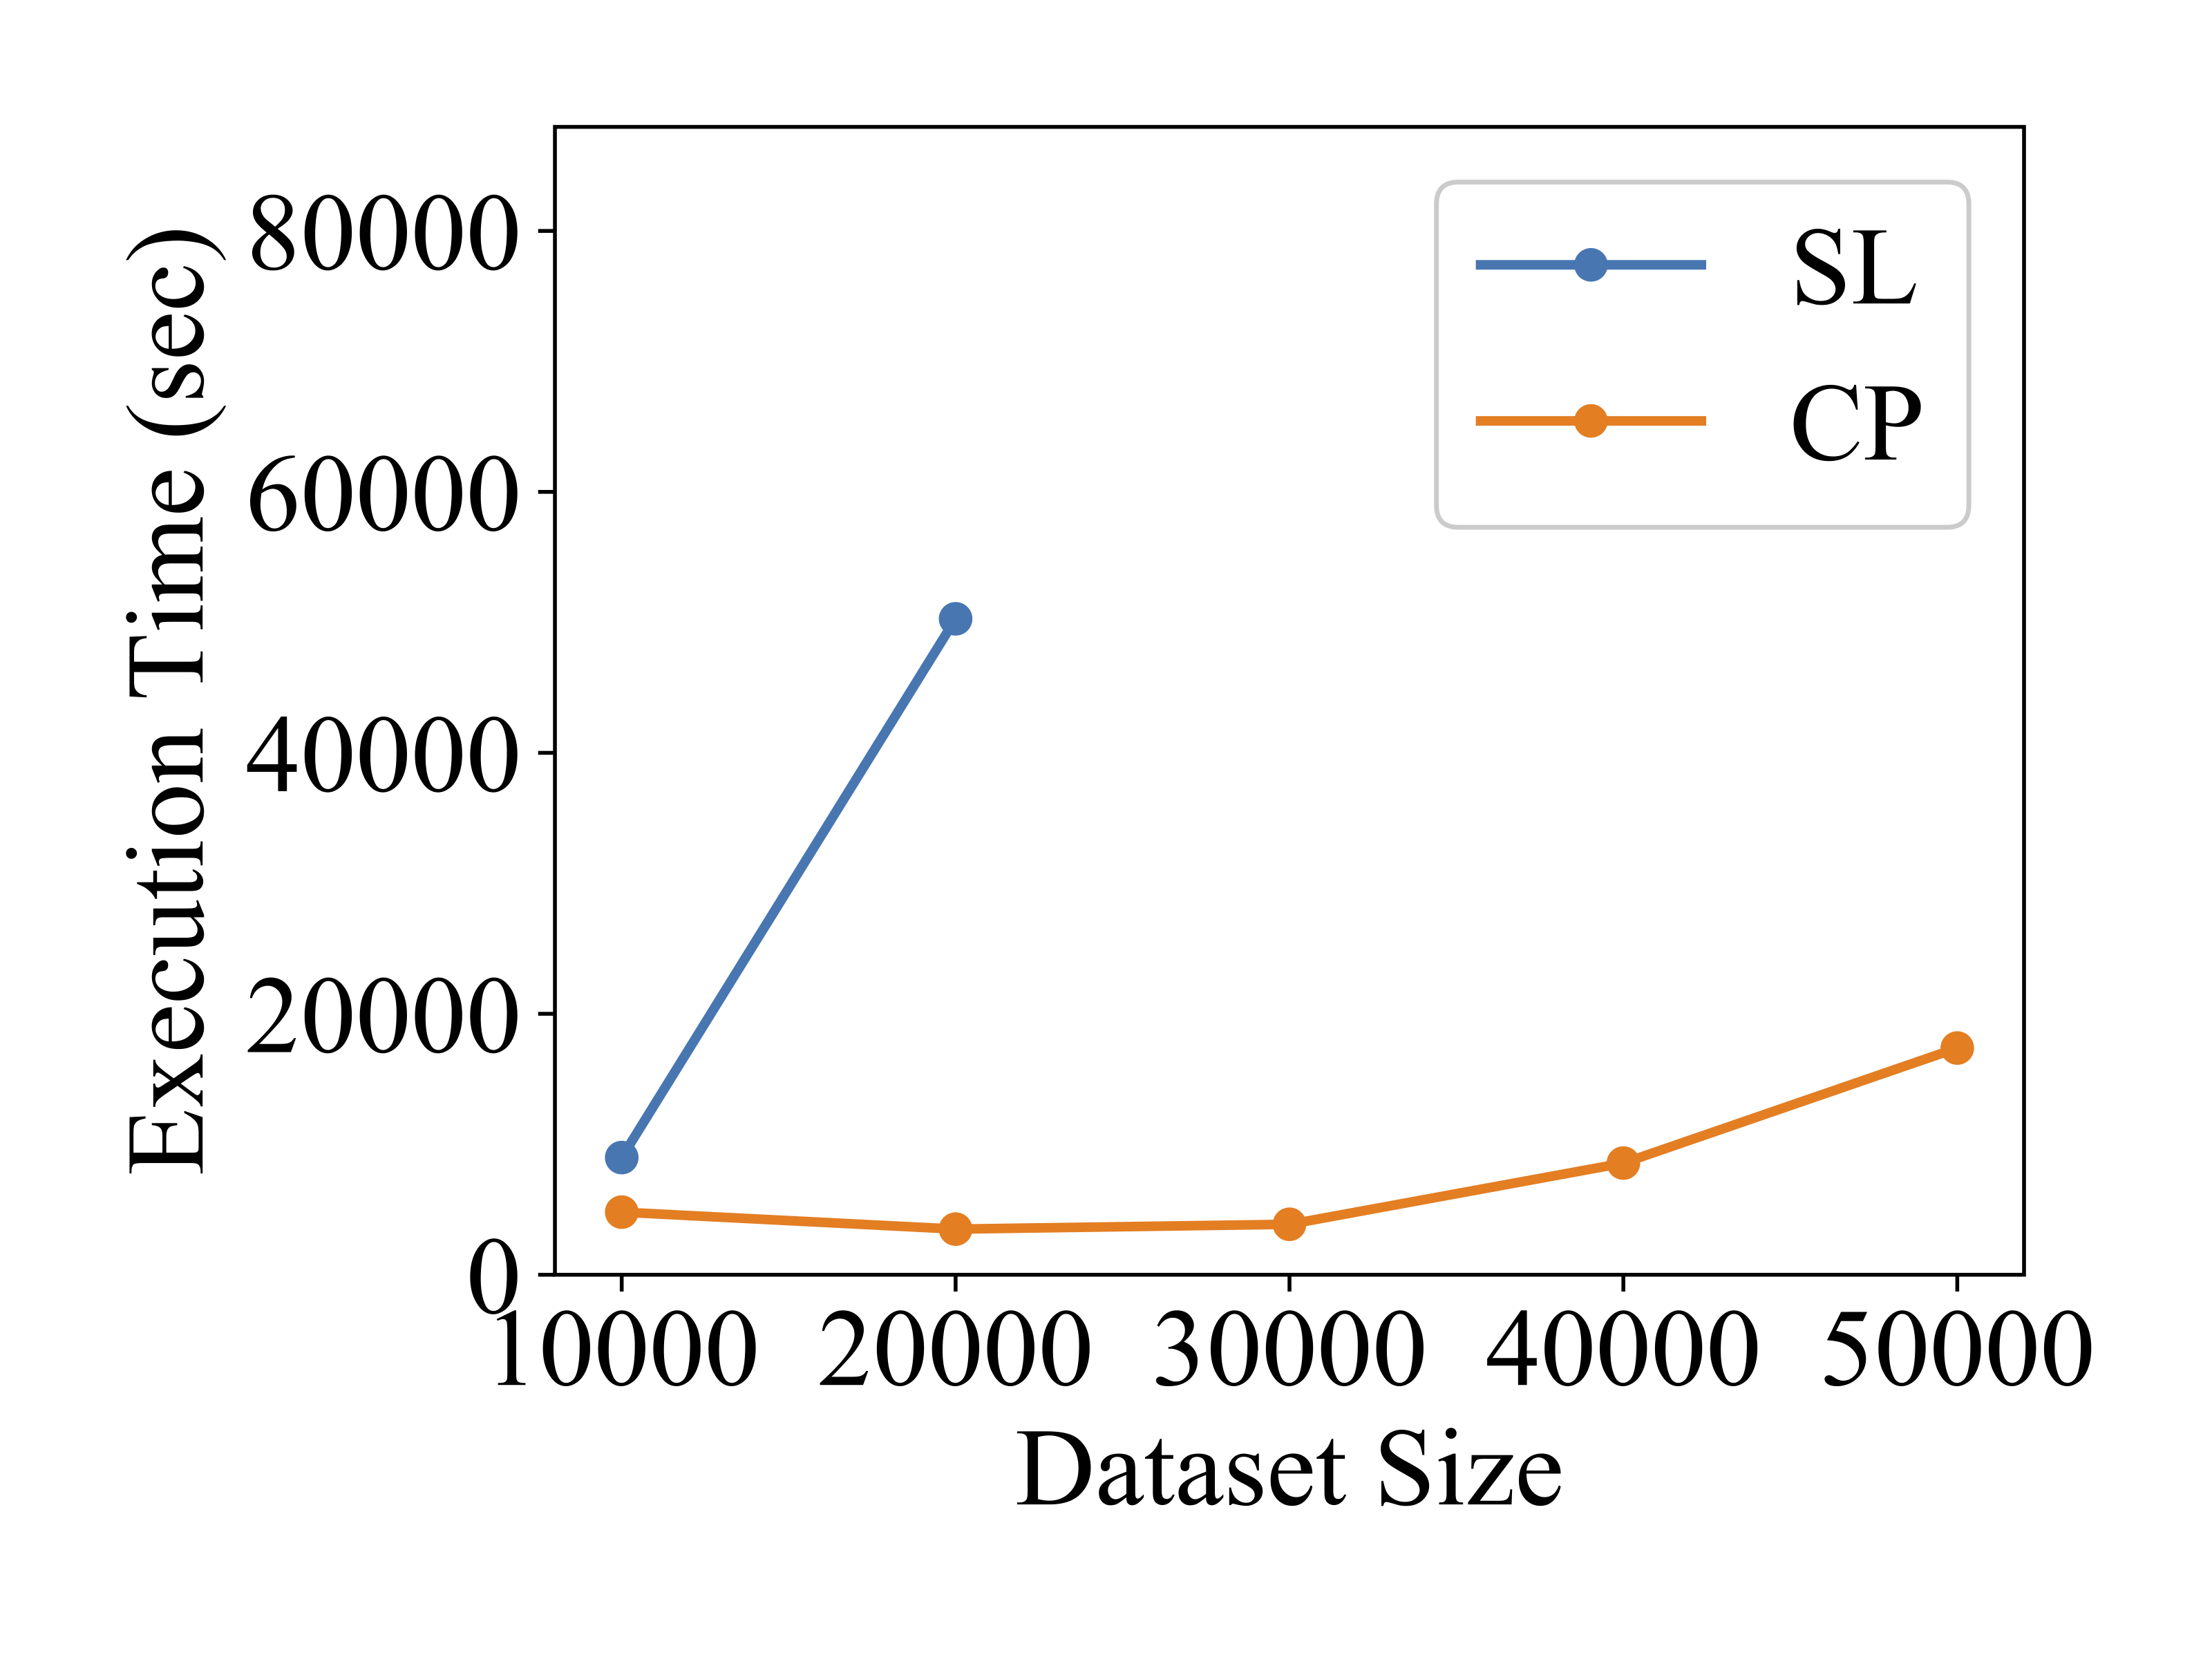
\includegraphics[trim=0.5cm 0.5cm 0.5cm 0.5cm, clip,width=0.45\textwidth]{figures/plots/bundles/varying_dataset_size.png}\label{subfig:var_dat_size}}
 \subfloat[Pair discovery]{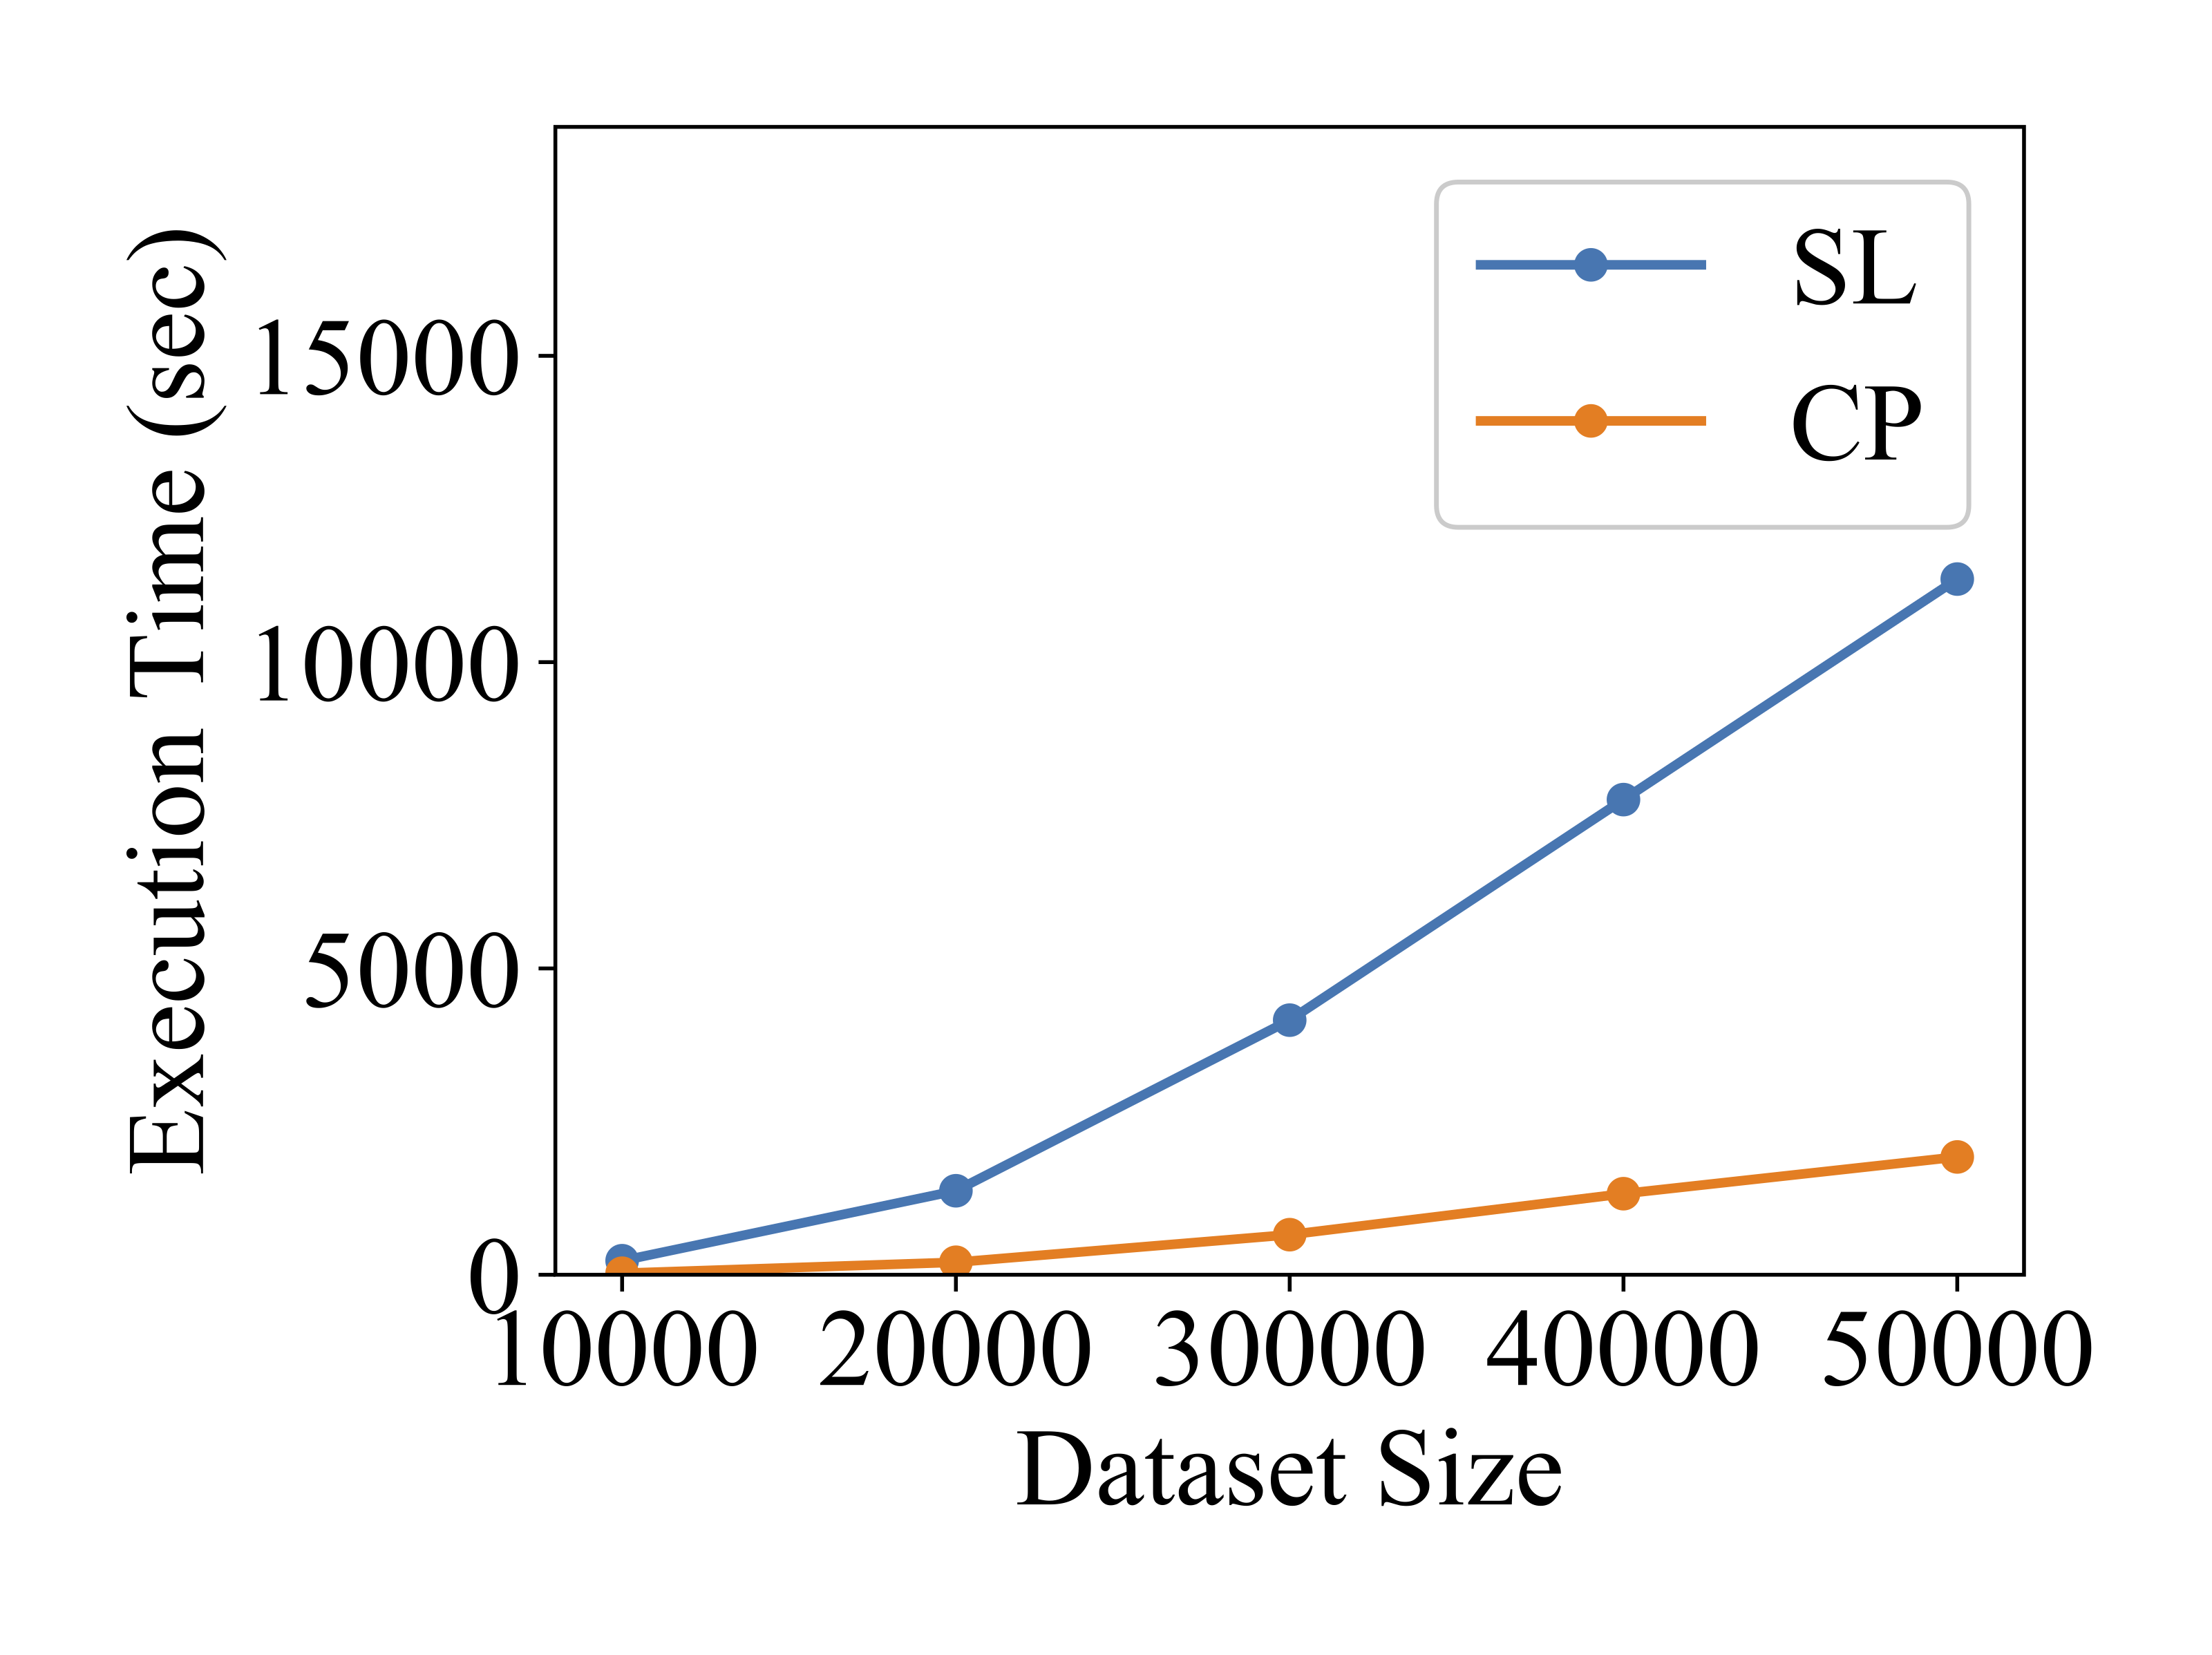
\includegraphics[trim=0.5cm 0.5cm 0.5cm 0.5cm, clip,width=0.45\textwidth]{figures/plots/pairs/varying_dataset_size.png}\label{subfig:var_dat_size_pairs}}
 \caption{Efficiency with varying numbers of time series.}
 \label{fig:exp4}
\end{figure}

\begin{table}[!ht]
\centering
\caption{Parameters for tests against synthetic data}
\begin{small}
\begin{tabular}{lc} 
\hline
{\em Parameter} &{\em Values} \\
\hline
Dataset Size & \textbf{10000}, 20000, 30000, 40000, 50000 \\
Time Series Length & 600, 700, \textbf{800}, 900, 1000 \\
$\delta$ (\% of time series length) & \textbf{2.5\%} \\
$\epsilon$ (\% of value range) & \textbf{0.2\%} \\
$\mu$ (\% of dataset size) & \textbf{1.25\%} \\
\hline
\end{tabular}
\end{small}
\label{tab:parameters2}
\end{table}

Figure \ref{fig:exp4} depicts the performance comparison between CP and SL algorithms for bundle and pair discovery. We omit cases where execution of an algorithm was taking more than 15 hours (cutoff). As illustrated in Figure \ref{subfig:var_dat_size}, an increase in the dataset size leads to a very abrupt deterioration of performance for the SL algorithm of up to several hours of execution for 20,000 time series. For larger dataset sizes, the execution time was significantly longer than the cutoff time. On the other hand, CP reports results in all cases. Its execution time increases for larger dataset sizes, but manages to finish in a few hours in the worst case (for 50,000 time series). It is worth noting that membership parameter $\mu$ is more relaxed for larger dataset sizes, as it is expressed in terms of percentage of the total number of time series in the dataset. This explains the slight improvement in performance  for dataset sizes of 20,000 and 30,000 for the CP method. In general, CP is more than an order of magnitude faster than SL, which also stands for the case of pair discovery, as illustrated in Figure \ref{subfig:var_dat_size_pairs}. As the number of time series in the dataset grows, it is natural that more pairs will be detected, hence the linear increase in the execution cost for the CP algorithm. Of course, baseline SL requires more time, as it must check many more combinations of time series.

\paragraph{Varying Time Series Length}
\begin{figure}[!ht]
 \centering
 \subfloat[Bundle discovery]{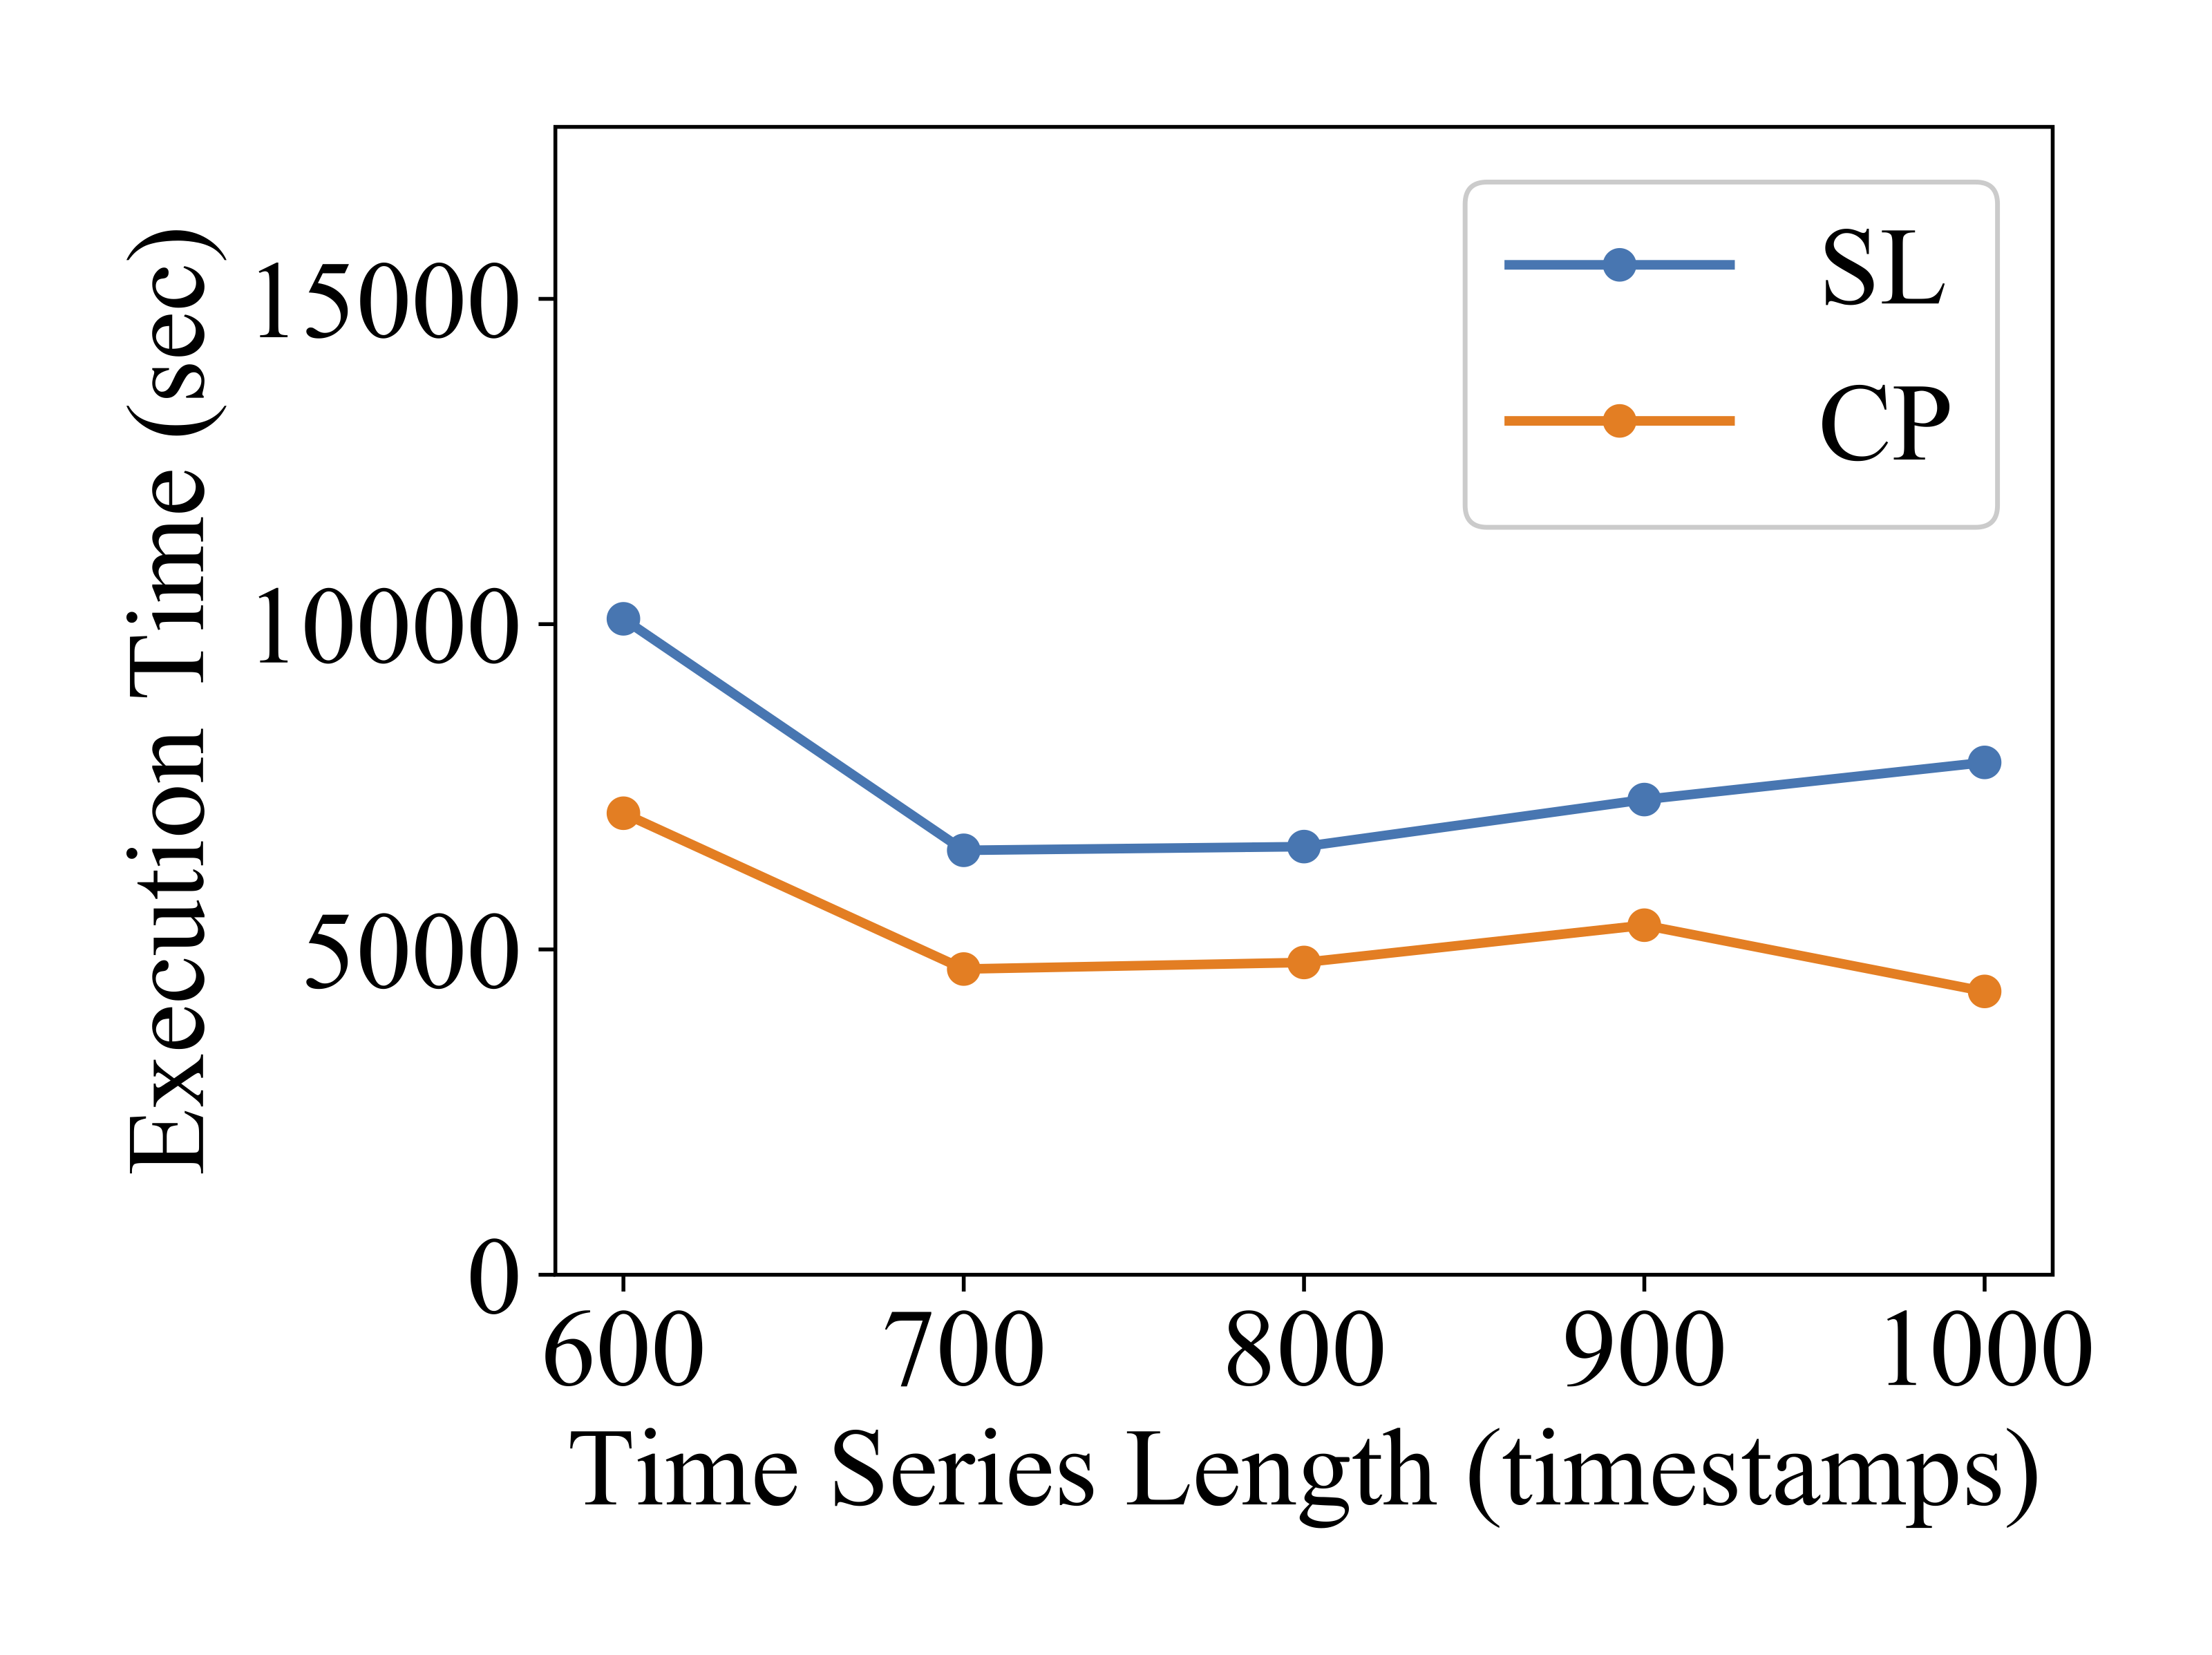
\includegraphics[trim=0.5cm 0.5cm 0.5cm 0.5cm, clip,width=0.45\textwidth]{figures/plots/bundles/varying_time_series_length.png}\label{subfig:var_ts_length}}
 \subfloat[Pair discovery]{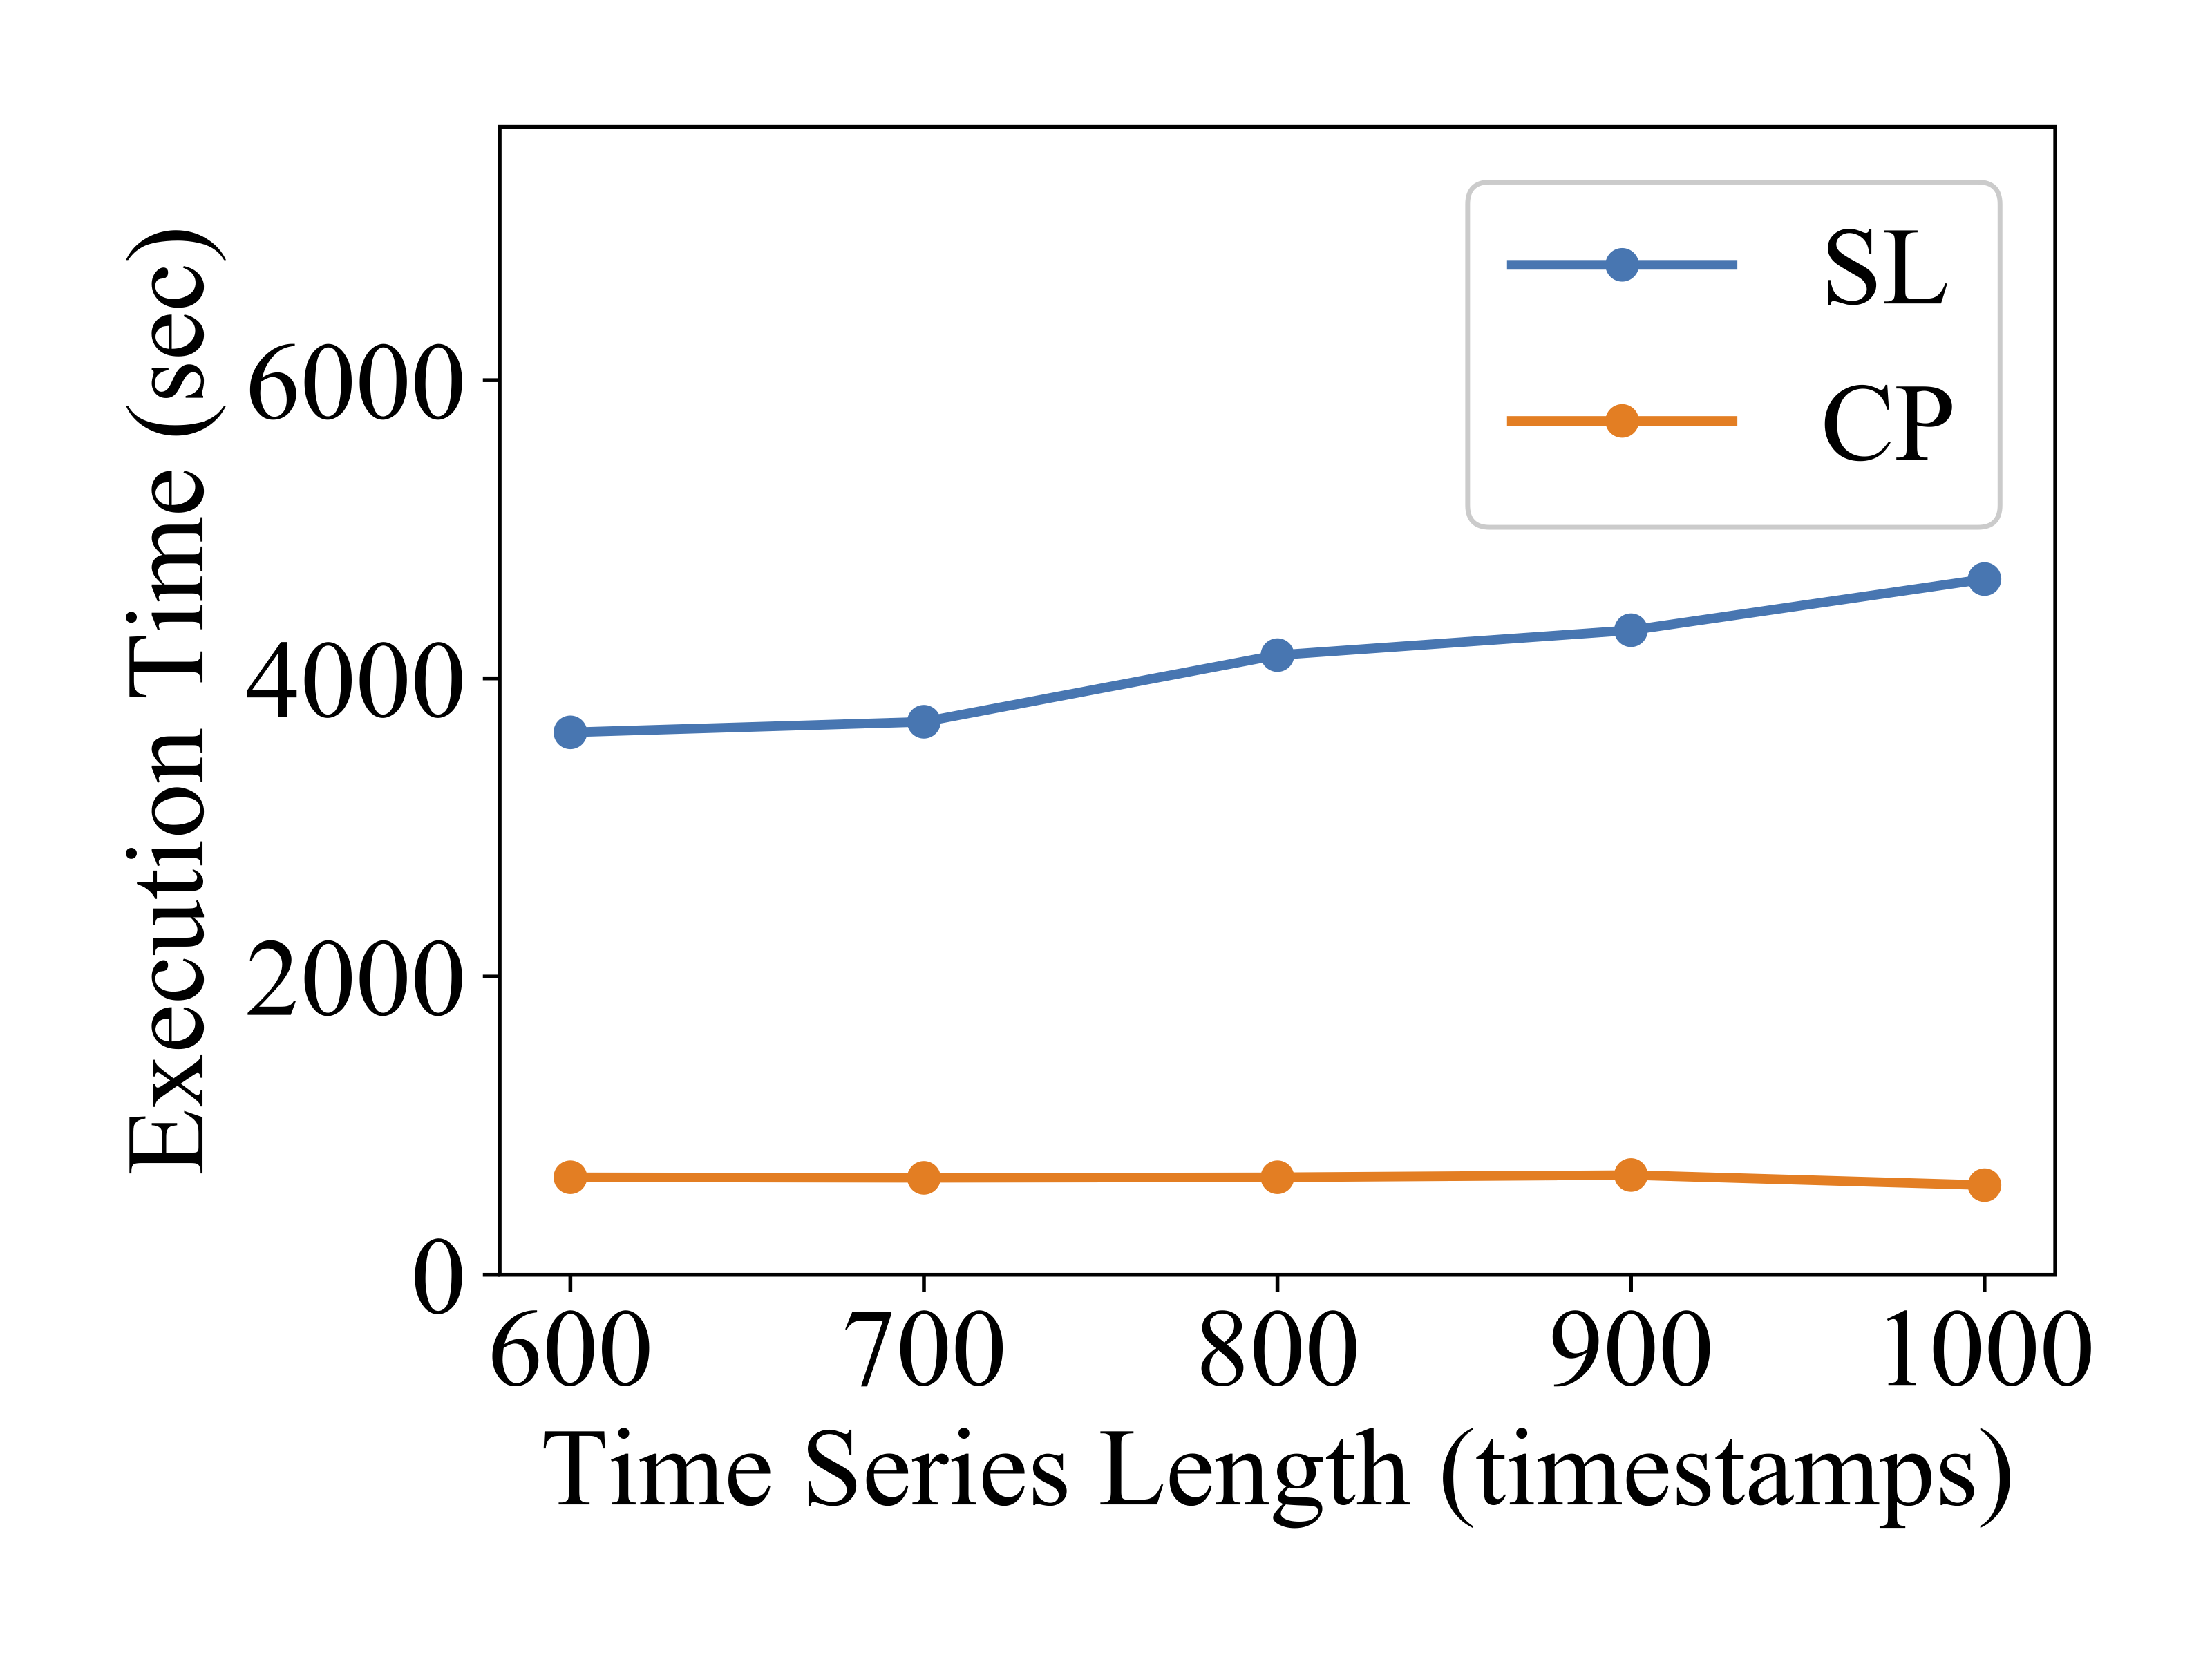
\includegraphics[trim=0.5cm 0.5cm 0.5cm 0.5cm, clip,width=0.45\textwidth]{figures/plots/pairs/varying_time_series_length.png}\label{subfig:var_ts_length_pairs}}
 \caption{Efficiency with varying length of time series.}
 \label{fig:exp5}
\end{figure}

For time series with increasing length (Figure~\ref{subfig:var_ts_length}), the CP algorithm for bundle discovery again constantly outperforms SL. Similarly to previous experiments, $\delta$ is expressed as a percentage of the time series length. We observe that the execution time initially decreases for both algorithms, as more bundles are pruned. However, as the time series length (and $\delta$) gets larger, the performance of both algorithms slightly worsens. Only in the case of 1,000 timestamps the execution time starts to drop for the CP algorithm due to the even larger $\delta$. This is not the case with the SL method, which has to evaluate more timestamps. Notice that the difference between the SL and CP algorithms is smaller, compared to the real dataset. This is due to the larger number of existing bundles in the synthetic dataset, which were detected on the checkpoints and had to be verified. Similar observations stand for pair discovery, with the CP algorithm significantly outperforming SL in all cases (Figure~\ref{subfig:var_ts_length_pairs}).